\documentclass[11pt]{article}
% packages
\usepackage[utf8]{inputenc}
\usepackage{geometry}
\usepackage[pdftex]{graphicx}
\usepackage{graphicx}
\usepackage{tabularx}
\usepackage{dsfont}
\usepackage{multirow}
\usepackage{amsmath,amsfonts,amssymb}
\usepackage{subcaption}
\usepackage{authblk}
\usepackage{placeins}
%hyperlinks options
\usepackage{hyperref}
\hypersetup{colorlinks=true,linkcolor=blue,filecolor=magenta,urlcolor=cyan,citecolor=cyan}
%bib options
\usepackage[backend=biber,style=authoryear,bibstyle=authoryear,natbib=true,
giveninits=true,uniquename=false,uniquelist=false,% firstinits=false,
maxcitenames=2,date=year, maxbibnames=99,url=false]{biblatex}
\geometry{left=20mm, top=20mm, right=20mm}
%float barrier
\usepackage{placeins}
 \addbibresource{Thèse.bib}
\title{Chapitre 3 : Analyse probabiliste des crues du Rhône à Beaucaire du XVI\textsuperscript{ème} siècle à aujourd'hui}
\author{Mathieu}


\begin{document}
\maketitle

\tableofcontents

\section{Introduction du chapitre}
	Quelques rappels d'intro aux méthodes d'analyse des crues histo:
	\cite{stedinger_flood_1986}\\
	Solutions quand le débit est connu\\
	Solution quand le débit n'est pas connu	\\
	Définition seuil et durée période histo\\
	%	plot positions (\citet{hirsch_techniques_1982}...)	\\
	Explication du concept de seuil de perception et de ses limites.\\
	durée de la période historique\\
	
	\paragraph{Méconnaissance du seuil}
	Le seuil de perception est un concept empirique qui ne prend une signification physique que dans certaines situations. Par exemple, imaginons une station hydrométrique dont la section n'a pas évolué au cours du temps et pour laquelle les débordements surviennent toujours au delà d'un même débit. Ces débordements (par exemple au-dessus d'une digue qui n'a subi aucune modification au cours du temps) laissent systématiquement une trace dans les écrits ou sur des infrastructures (marques de crue) suite aux dommages occasionnés. Cette situation parfaite existe rarement et le concept de seuil de perception peut être mis à mal par une variabilité temporelle de la perception des crues par les populations ripariennes. Néanmoins, l'utilisation du concept de seuil de perception est très souvent obligatoire pour exploiter les données de crues historiques. 
	
	\paragraph{Méconnaissance de la durée histo}Cette durée est pourtant importante dans le calcul de la binomiale. Il est erroné de considérer que la période historique démarre à la première crue et cela peut entrainer une sur-estimation de la fréquence d'occurrence. Plusieurs méthodes existent dans la littérature pour calculer cette durée et se basent sur (A COMPLETER...). 
		
\section{Méthodes d'analyse probabiliste d'un échantillon mixte de crues}
	
	
	\subsection{Concepts de base et hypothèses}
	
	\paragraph{} 
	
		L'utilisation d'occurrences de crues historiques pour l'analyse fréquentielle nécessite a minima l'hypothèse suivante : le débit de tous les événements de crue qui ont laissé une trace est supérieur à un seuil de perception. Cela implique que pour toutes les années de la période historique sans mention de crue, on fait l'hypothèse que le débit inconnu a été inférieur au seuil de perception. Aussi, l'échantillon des crues supérieures au seuil de perception est supposé exhaustif. Il existe des méthodes d'analyse pour lesquelles il n'est pas nécessaire de connaitre précisément le débit des événements supérieurs au seuil de perception (voir notamment \citet{stedinger_flood_1986}). Le nombre de dépassements d'un seuil de perception pour une durée donnée est une information qui peut être exploitée en l'état. Ainsi, il faut considérer un échantillon mixte, composé d'une part de débits enregistrés en continu et d'autre part d'un nombre d'occurrences de crues supérieures à un seuil de perception. 
			
		\paragraph{}
		De manière similaire au Chapitre 1 (REF), on suppose que le débit maximum annuel des périodes continues et historiques $Q$ est une variable aléatoire $iid$ qui suit une distribution GEV, de paramètres $\boldsymbol{\theta} = (\mu,\sigma,\xi)$ (respectivement : position, échelle, forme). Pour simplifier, on suppose ici que le paramètre de forme $\xi$ est différent de zéro (forme Gumbel). Ainsi, on a la fonction de répartition de la GEV : $F(x;\boldsymbol{\theta}) = e^{-(1-\xi(\frac{x - \mu}{\sigma}))^{1/\xi}}$. Les débits de l'échantillon de maximum annuels enregistrés en continu pendant $j$ années $\boldsymbol{q}= (q_t)_{t=1,...,j}$ sont ici supposés parfaitement connus et dans un premier temps non affectés d'une quelconque incertitude. L'échantillon historique est composé de $k$ événements ayant dépassé le seuil de perception $S$ sur une période de $n$ années. Le seuil de perception n'a donc pas été dépassé pour les $n-k$ années restantes. Ainsi, la probabilité de dépassement du seuil peut s'écrire :
		
		\begin{equation}
			\pi = \biggl( 1 - F(S;\boldsymbol{\theta})\biggl) = 1 - e^{-\biggl(1-\xi\bigl(\frac{S-\mu}{\sigma}\bigl)\biggl)^{1/\xi} }		
		\end{equation}
			 
	On suppose que $k$, le nombre de dépassements du seuil de perception, peut être estimé par une loi binomiale de paramètres $n$ et $\pi$, soit $\mathcal{B}(n,\pi)$. On peut alors écrire la fonction de vraisemblance (équation \ref{eq:Gev_Binom}) qui est fonction d'un échantillon mixte de données composé des débits maximum annuels de la période continue $(q_t)_{t=1,...,j}$ et du nombre de dépassements du seuil de perception $k$ durant la période historique $n$ :
		
			\begin{equation}
			L(\boldsymbol{\theta} ; \boldsymbol{q}, k) = \underbrace{\prod_{t=1}^j f\left(q_t;\boldsymbol{\theta}\right)}_{\mathrm{a}} \underbrace{\left\{\left(\begin{array}{l}
			n \\
			k
			\end{array}\right) F\left(S;\boldsymbol{\theta}\right)^{n-k}\left[1-F\left(S;\boldsymbol{\theta}\right)\right]^k\right\}}_{\mathrm{b}} \\
			\label{eq:Gev_Binom}
			\end{equation}
			
			Ici, le terme $\mathrm{a}$ représente la vraisemblance pour les données continues et le terme $\mathrm{b}$ pour les données historiques. L'application de la formule de Bayes permet de calculer la distribution a posteriori des paramètres $\boldsymbol{\theta}$ sachant les données :
			
			\begin{equation}
				p(\boldsymbol{\theta} \mid \boldsymbol{q},k) \propto L(\boldsymbol{\theta};\,\boldsymbol{q},k) p(\boldsymbol{\theta})
				\label{eq:BayesBinom}
			\end{equation}
	
		Le terme $P(\boldsymbol{\theta})$ représente ici la distribution a priori des paramètres qu'il faudra éliciter. La distribution a posteriori est explorée via une méthode bayésienne MCMC (notamment décrite par \citet{coles_classical_2001}). Cette distribution a posteriori représente l'incertitude d'échantillonnage du modèle par $r$ jeux de paramètres : $\boldsymbol{\Theta} = (\boldsymbol{\theta_1},...,\boldsymbol{\theta_r})$. Le jeu de paramètres qui maximise la distribution a posteriori est appelé maxpost et s'écrit $\boldsymbol{ \hat{\theta} }$.
	
	
%	\paragraph{Description difficultés de détermination du seuil et durée historique}
%	Complexité de déterminer le seuil\\
%	Complexité de déterminer la durée de la période historique \citep{prosdocimi_german_2018}). 			Attention aux confusions entre date de début de la période et durée de la période. \\

	
	\subsection{Propagation de l'incertitudes hydrométriques des mesures systématiques (modèle A)}
	
	\paragraph{}
	Dans la section précédente, l'incertitude des débits maximum annuels de la période continue est supposée négligeable. Cette incertitude pouvant atteindre 30 \% à Beaucaire (REF Chap 1), il semble pragmatique de la considérer. Comme décrit dans la section REF du Chapitre 1, cette incertitude hydrométrique est représentée par $s = 500$ réalisations : $(q_t^{(i)})_{t=1,...,j;\,i=1,...,s}$. Elle peut être propagée aux estimations des paramètres de l'équation \ref{eq:Gev_Binom} en estimant un jeu de paramètres pour chacune des $s$ réalisations, soit $(\boldsymbol{\theta}
	^{(i)})_{i=1,...,s}$. Au total, $r \times s$ jeux de paramètres sont estimés et représentent l'effet combiné de l'incertitude d'échantillonnage et de l'incertitude hydrométrique des données continues, on a donc $(\boldsymbol{\theta}^{(i)}_p)_{p=1,...,r;\, i=1,...,s}$. Le jeu de paramètres le plus probable est calculé en utilisant l'échantillon maxpost de débits maximum annuels (CHAPITRE 1) sur lequel on estime le jeu de paramètres maxpost de l'équation \ref{eq:Gev_Binom}. Le modèle décrit ci-dessus sera appelé "modèle A". La propagation des incertitudes hydrométriques de la période continue telle que décrite ici sera effectuée similairement pour les trois modèles définis dans les sections suivantes.
	
	\subsection{Seuil de perception incertain (modèle B)}
	
		\paragraph{}
		Afin de considérer dans le modèle proposé une prise en compte pragmatique de la méconnaissance du seuil de perception, il est possible de considérer ce seuil comme étant un paramètre à part entière du modèle. Il ne s'agit pas ici de considérer un seuil de perception variable au cours du temps, quoi que de nombreux exemples dans la littérature font l'hypothèse de plusieurs seuils de perception successifs dont le débit est différent (REFS). Un seul seuil de perception est ici considéré pour l'ensemble de l'échantillon, mais sa valeur est incertaine et est déterminée par le modèle. L'impact de la méconnaissance du seuil est ainsi répercuté sur l'incertitude des résultats. Dans la section précédente, le seuil de perception faisait déjà partie du modèle (équation \ref{eq:Gev_Binom}), mais sa valeur était supposée connue, ce qui n'est ici plus le cas. La vraisemblance s'écrit alors : 
		
				\begin{equation}
				L(\boldsymbol{\theta}, S ; \boldsymbol{q}, k) =\prod_{t=1}^j f\left(q_t;\boldsymbol{\theta}\right) \left\{\left(\begin{array}{l}
				n \\
				k
				\end{array}\right) F\left(S;\boldsymbol{\theta}\right)^{n-k}\left[1-F\left(S;\boldsymbol{\theta}\right)\right]^k\right\} \\
				\label{eq:Gev_Binom_uS}
				\end{equation}
				
		On peut alors écrire une nouvelle distribution a posteriori : 			
				
				\begin{equation}
					p(\boldsymbol{\theta}, S \mid \boldsymbol{q},k) \propto L(\boldsymbol{\theta},S;\,\boldsymbol{q},k) p(\boldsymbol{\theta},S)
					\label{eq:Bayes_uS}
				\end{equation}
			
		Les distributions de paramètres a posteriori de ce modèle reflètent donc l'incertitude hydrométrique de la période continue, l'incertitude d'échantillonnage, ainsi que l'incertitude du seuil de perception. Ce modèle sera nommé "modèle B" dans les sections suivantes.
		

	\subsection{Durée de la période historique incertaine (modèle C)}
	
		\paragraph{}
		L'équation \ref{eq:Gev_Binom} repose à la fois sur le fait que le seuil de perception $S$ et la durée de la période historique $n$ sont connus. De la même manière que décrit à la section précédente pour le seuil, la durée (et donc l'année qui marque le début) de la période historique peut être complexe à déterminer. Nous proposons ici de considérer la durée de la période historique comme étant un paramètre à part entière du modèle. Ici, le seuil de perception est en revanche supposé parfaitement connu. La vraisemblance s'écrit alors : 
		 
				\begin{equation}
				L(\boldsymbol{\theta}, n ; \boldsymbol{q}, k) = \prod_{t=1}^j f\left(q_t;\boldsymbol{\theta}\right) \left\{\left(\begin{array}{l}
				n \\
				k
				\end{array}\right) F\left(S;\boldsymbol{\theta}\right)^{n-k}\left[1-F\left(S;\boldsymbol{\theta}\right)\right]^k\right\} \\
				\label{eq:Gev_Binom_uN}
				\end{equation}
				
		On peut alors exprimer une nouvelle distribution a posteriori :
		
				\begin{equation}
					p(\boldsymbol{\theta}, n \mid \boldsymbol{q},k) \propto L(\boldsymbol{\theta},n;\,\boldsymbol{q},k) p(\boldsymbol{\theta},n)
					\label{eq:Bayes_uN}
				\end{equation}
			
		Ainsi, la méconnaissance de la durée de la période historique est prise en compte par le modèle et est reportée dans l'incertitude des résultats. Ce modèle sera nommé "modèle C" dans les sections suivantes. 
	
	\subsection{Seuil de perception et durée de la période historique incertains (modèle D)}
	
	\paragraph{}
	Enfin, on peut également considérer un modèle qui représente en même temps la méconnaissance du seuil de perception $S$ et de la durée de la période historique $n$. Sa vraisemblance s'écrit :  
	
					\begin{equation}
			L(\boldsymbol{\theta}, S, n ; \boldsymbol{q}, k) = \prod_{t=1}^j f\left(q_t;\boldsymbol{\theta}\right) \left\{\left(\begin{array}{l}
			n \\
			k
			\end{array}\right) F\left(S;\boldsymbol{\theta}\right)^{n-k}\left[1-F\left(S;\boldsymbol{\theta}\right)\right]^k\right\} \\
			\label{eq:Gev_Binom_SN}
			\end{equation}
		
		La distribution a posteriori de ce modèle s'écrit :
					
			\begin{equation}
				p(\boldsymbol{\theta}, S, n \mid \boldsymbol{q},k) \propto L(\boldsymbol{\theta},S, n;\,\boldsymbol{q},k) p(\boldsymbol{\theta},S, n)
				\label{eq:Bayes_uSN}
			\end{equation}

	Il sera nommé "modèle D" dans les sections suivantes. 
	
	\subsection{Modèle E : Censure}
	\paragraph{} Est-il nécessaire d'écrire la vraisemblance de ce modèle ? CF \citet{stedinger_flood_1986}

	\subsection{Distribution empirique d'un échantillon mixte}
	
%	(HIRSCH 1987) et étude Rhin de Michel. 	
		\paragraph{} Le classement en fréquence des crues dans le cas d'un échantillon mixte peut poser problème, notamment quand le débit des crues historiques n'est pas connu, n'ayant d'autre information que le dépassement d'un seuil de perception. \citet{hirsch_probability_1987} propose une méthode pour le classement en fréquence d'un échantillon mixte quand le débit des crues est connu. Pour un échantillon continu de crues classé par valeurs décroissantes : $q(1) \geq ... \geq q(j)$, la fréquence empirique au dépassement s'écrit : $f_i = P(\boldsymbol{Q} > q(i)) = \frac{i-\alpha}{j+1-2\alpha}$. Nous prenons ici $\alpha = 0.5$ (REF HAZEN). \\
		Pour un échantillon mixte composé d'un échantillon continu de $j$ débits maximum annuels et de $k$ crues historiques supérieures à un seuil $S$ couvrant $n$ années, il faut raisonner sous la forme de deux sous-échantillons. Le nombre de crues supérieures au seuil $S$ sur la période complète est ici noté $NS$, et la durée de la période complète correspond à $j + n$ années. On a d'après \citet{hirsch_probability_1987} :
		
		\begin{equation}	
		P(\boldsymbol{Q} > q(i)) = \begin{cases}\frac{i-\alpha}{NS+1-2 \alpha} \frac{NS}{j+n}, & i=1, \ldots, NS \\ \frac{NS}{j+n}+\frac{j+n-NS}{j+n} \frac{(i-NS-\alpha)}{(j-NS+1-2\alpha)}, & i=NS+1, \ldots, j+k\end{cases}
		\label{eq:FreqHisto}	
		\end{equation}
	
	Lorsque le débit des crues historiques est connu, on peut classer l'ensemble des crues sup-seuil (de la période continue et historique) par ordre décroissant en leur attribuant le rang $i$. Lorsque le débit des crues historiques n'est pas connu, il n'est pas possible de classer l'échantillon de crues sup-seuil. Une manière de contourner ce problème est de tirer aléatoirement le rang $i$ de l'ensemble des crues sup-seuil. Ce classement n'est est aléatoire mais permet d'affecter une fréquence empirique aux crues. Ainsi, on peut comparer la fréquence empirique des observations de crues aux ajustements statistiques décrits dans les sections précédentes afin de vérifier leur cohérence. 
		
\section{Données disponibles}

	\subsection{Échantillon mixte de crues du Rhône à Beaucaire}
	\paragraph{} Les données de crues du Rhône à Beaucaire sont constituées de deux échantillons. Premièrement, un échantillon continu de débits maximum annuels mesurés de 1816 à 2020. Ces débits ont été estimés au Chapitre 1 (REF) et leur incertitude hydrométrique est représentée par 500 réalisations de l'échantillon. Deuxièmement, une collection de témoignages de crues historiques de 1500 à 1816, classées en deux catégories tel que décrit au chapitre 2 (REF). Les seuils de perception correspondant aux catégories ne sont pas précisément connus, mais on suppose que le seuil $S3$ qui correspond aux crues des catégories C3 et C4 se situe aux alentours de 7000 $m^3/s$, et le seuil $S4$ qui correspond aux crues de la catégorie C4 uniquement se situe aux alentours de 9000 $m^3/s$ (VALEURS DEFINIES AU CHAP 2). La figure \ref{fig:EchMixte} présente l'ensemble des données disponibles. 
	
	\begin{figure}[h]
		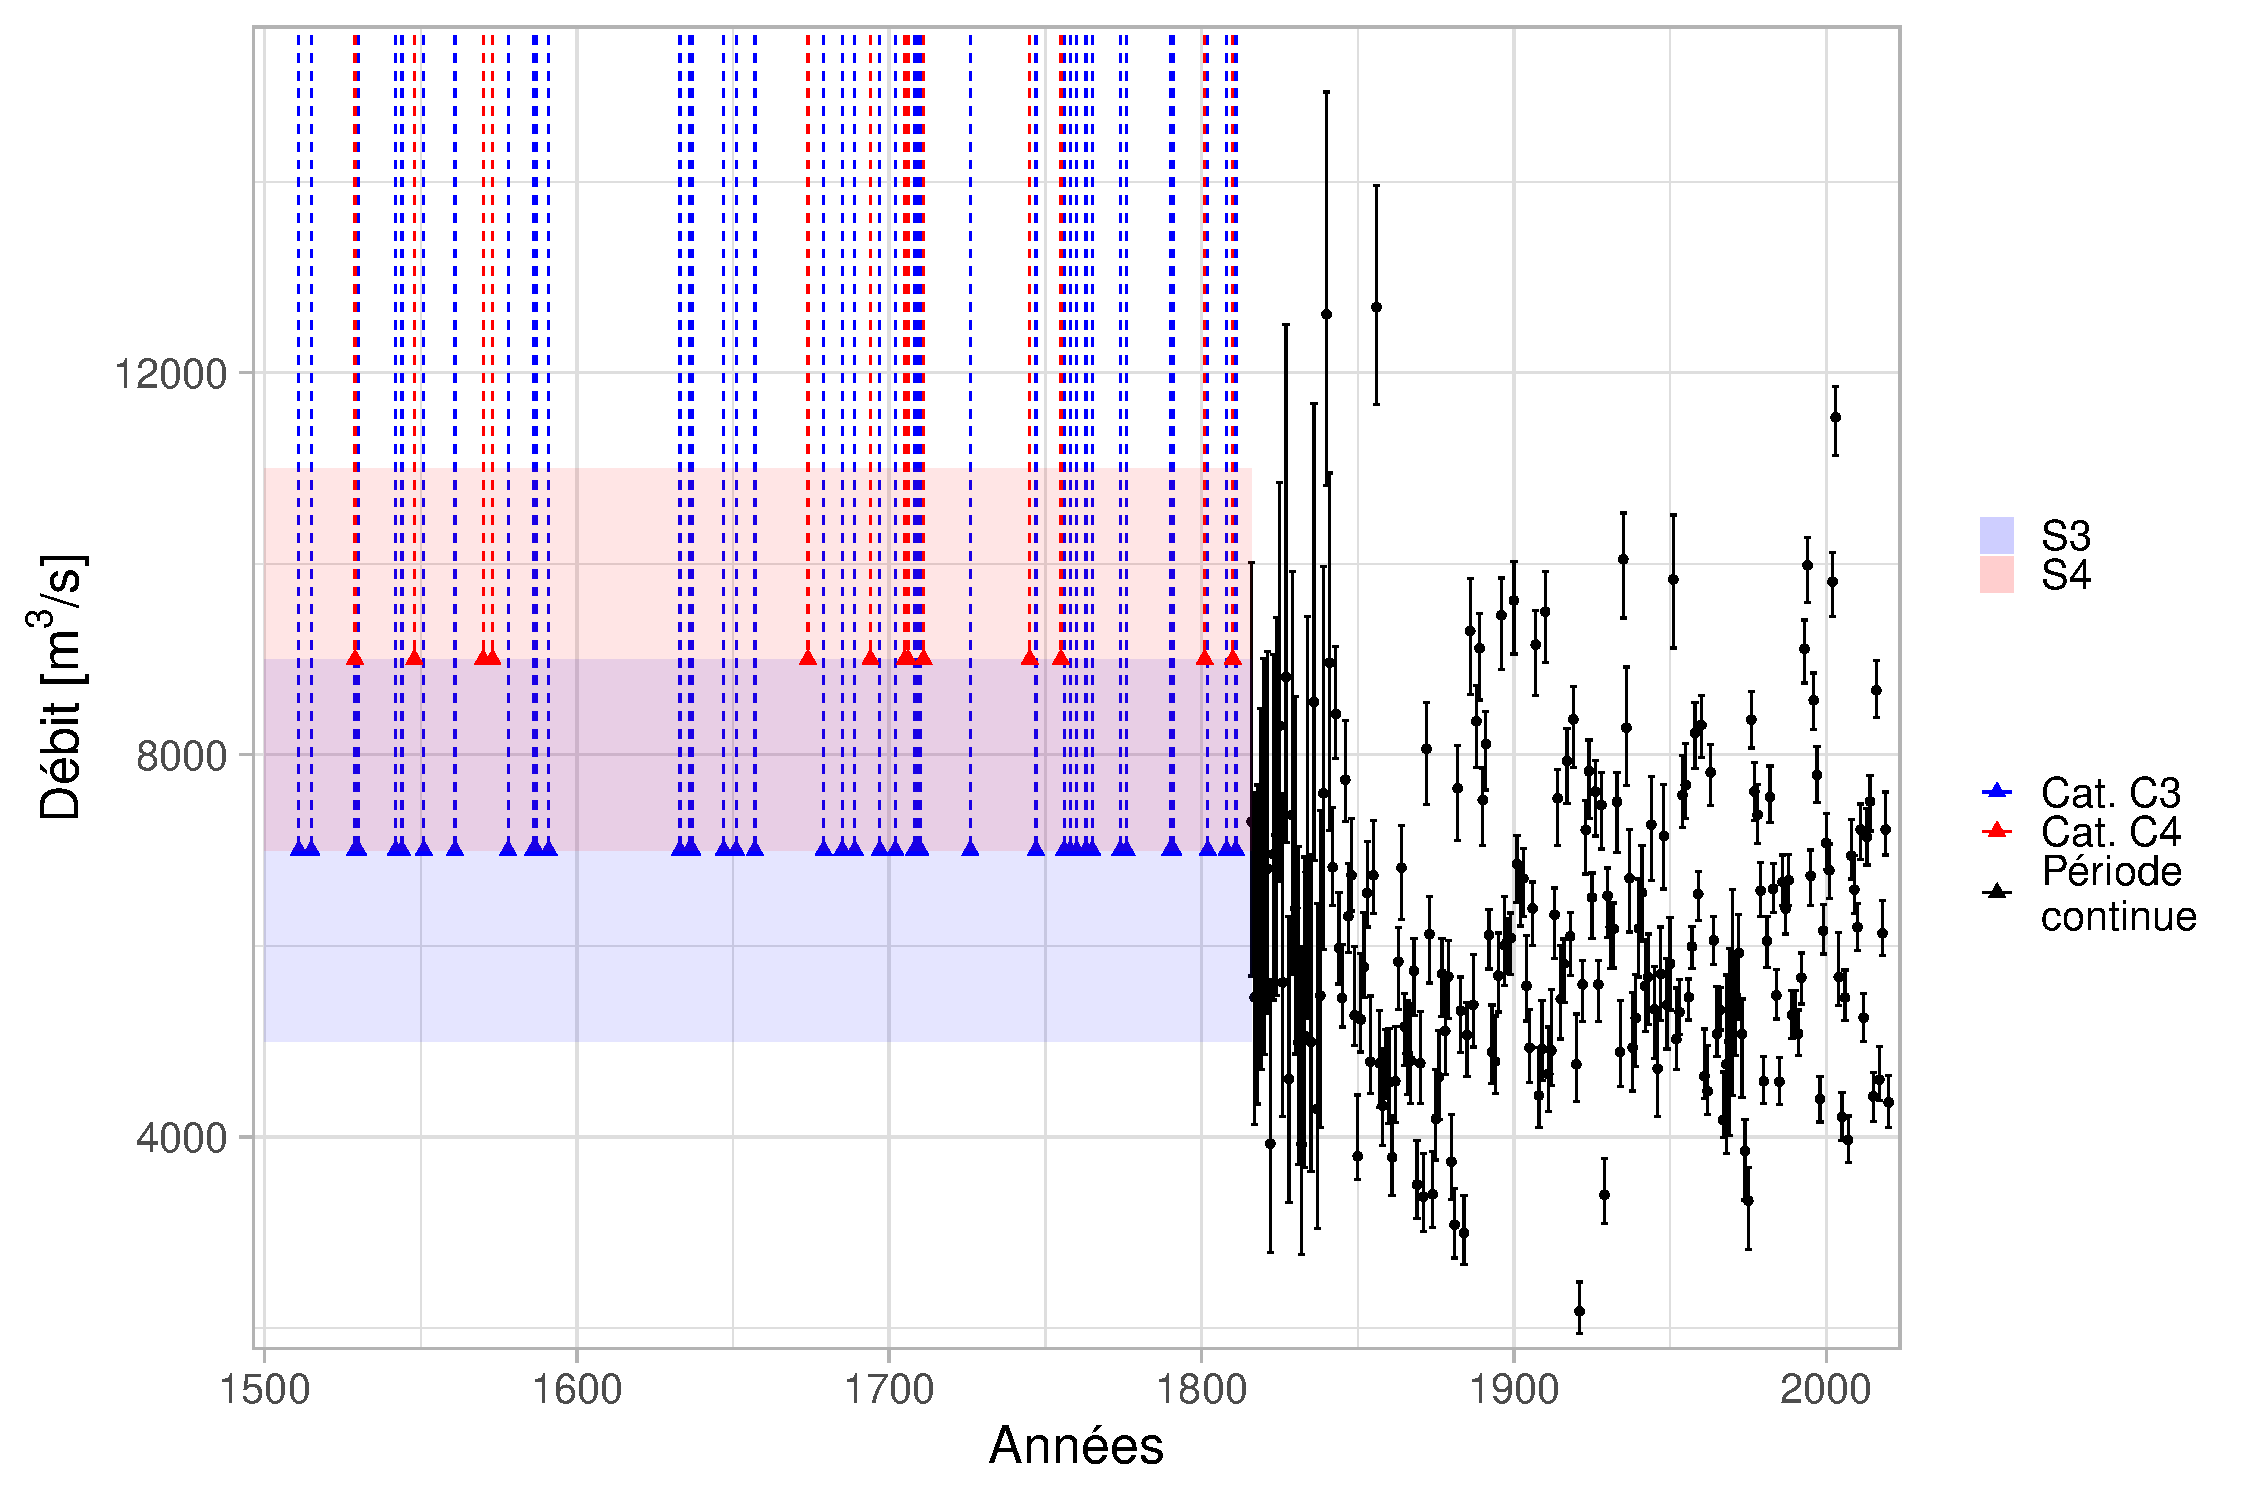
\includegraphics[width=.9\linewidth]{Figures/EchMixteBcr.pdf}	
		\caption{Échantillon de crues du Rhône à Beaucaire. L'incertitude à 95\% autour des seuils de perception est représentée par les bandeaux bleu et rouge ("S3" et "S4)}
		\label{fig:EchMixte}
	\end{figure}
	

	\subsection{Homogénéité des données}
	\paragraph{} L'homogénéité des données est un pré-requis essentiel à l'analyse fréquentielle des crues en contexte stationnaire, car cette dernière repose sur l'hypothèse que les variables étudiées sont dites $iid$ (indépendantes et identiquement distribuées). C'est-à-dire que les processus statistiques pouvant être utilisés pour modéliser la distribution des crues ne changent pas dans le temps, et que pour une station donnée, une même distribution peut être utilisée pour modéliser les crues du XVI\textsuperscript{ème} et du XXI\textsuperscript{ème} siècle. Étant donné que deux types d'échantillons sont utilisés, deux types de tests statistiques sont utilisés pour étudier l'homogénéité de ces échantillons. 

	\subsubsection{Données continues}
	
	\paragraph{} Trois tests seront utilisés pour qualifier l'homogénéité de l'échantillon de données continues : Le test de Pettitt (REF) et le test développé par \citep{darienzo_detection_2021-1} qui permettent de détecter des ruptures dans les séries temporelles, ainsi que le test de Mann-Kendall (REF) qui permet de détecter des tendances. Les ruptures sont des changements soudains (i.e. les données ont une distribution différente avant et après un instant $t$), tandis que les tendances représentent des changements progressifs dans la distribution des données au cours du temps. Parmi ces trois tests, seul le test de  \citep{darienzo_detection_2021-1} permet de considérer l'incertitude des données d'entrée. Elle est ici représentée par 500 réalisations possibles de la série temporelle des débits maximum annuels à Beaucaire déterminées au Chapitre 1 (REF).
	
	\paragraph{} La p-value des tests de Pettitt et Mann-Kendall appliqués à la série maxpost des débits maximum annuels à Beaucaire est respectivement de 0.15 et 0.41. Au risque d'erreur 5\%, on peut don conclure qu'il n'existe pas de tendance ou de rupture dans la série. Il faut cependant s'assurer que ce résultat est toujours vrai lorsque l'on considère les incertitudes de la série.
			
	\paragraph{} L'application du test de \citep{darienzo_detection_2021-1} à la série de débits maximum annuels avec incertitude a conclu qu'aucune rupture n'existait dans les données, quelque soit le critère de segmentation considéré (AIC, BIC, HQC ou DIC). 
	
	\paragraph{} Afin de d'étudier l'existence de tendances dans la série en considérant les incertitudes, le test de Mann-Kendall a été appliqué aux 500 réalisations possibles. Seulement 20\% des 500 p-values calculées sont inférieures à 0.05. Au risque d'erreur 5\%, on peut alors conclure que seulement 20\% des 500 réalisations de la série comportent une tendance. On peut calculer une valeur théorique ... A quelle valeur faudrait-il s'attendre pour considérer que c'est homogène (Benjamin ?) 
	
	\paragraph{} L'échantillon de données continues peut être considéré homogène suite aux tests statistiques réalisés. 
	
		
	\subsubsection{Données historiques}
	
	\paragraph{} Les données pré-enregistrements continus sont ici utilisés comme étant des occurrences de crues supposées supérieures à un seuil. Comme décrit par \citet{lang_towards_1999}, la fréquence des occurrences de crues sup-seuil est supposée suivre un processus de Poisson. Afin de vérifier l'homogénéité des occurrences sup-seuil, il est possible de calculer un intervalle de confiance autour du nombre cumulé de crues découlant du processus de Poisson. Si les occurrences de crues cumulées "sortent" de cet intervalle de confiance, alors leur fréquence d'occurrence est supposée non-stationnaire. 
	
	\paragraph{} Ces intervalles de confiance ont été calculés pour l'échantillon de crues pré-enregistrements continus du Rhône à Beaucaire. Le début de la période historique est supposé débuter en 1500 et se termine à l'année des premiers enregistrements continus de hauteur d'eau, en 1816. Les deux échantillons testés ici reflètent deux seuils de perception, $S3$ et $S4$, et on a $S3 < S4$. 

	\begin{figure}[h]
		\centering
		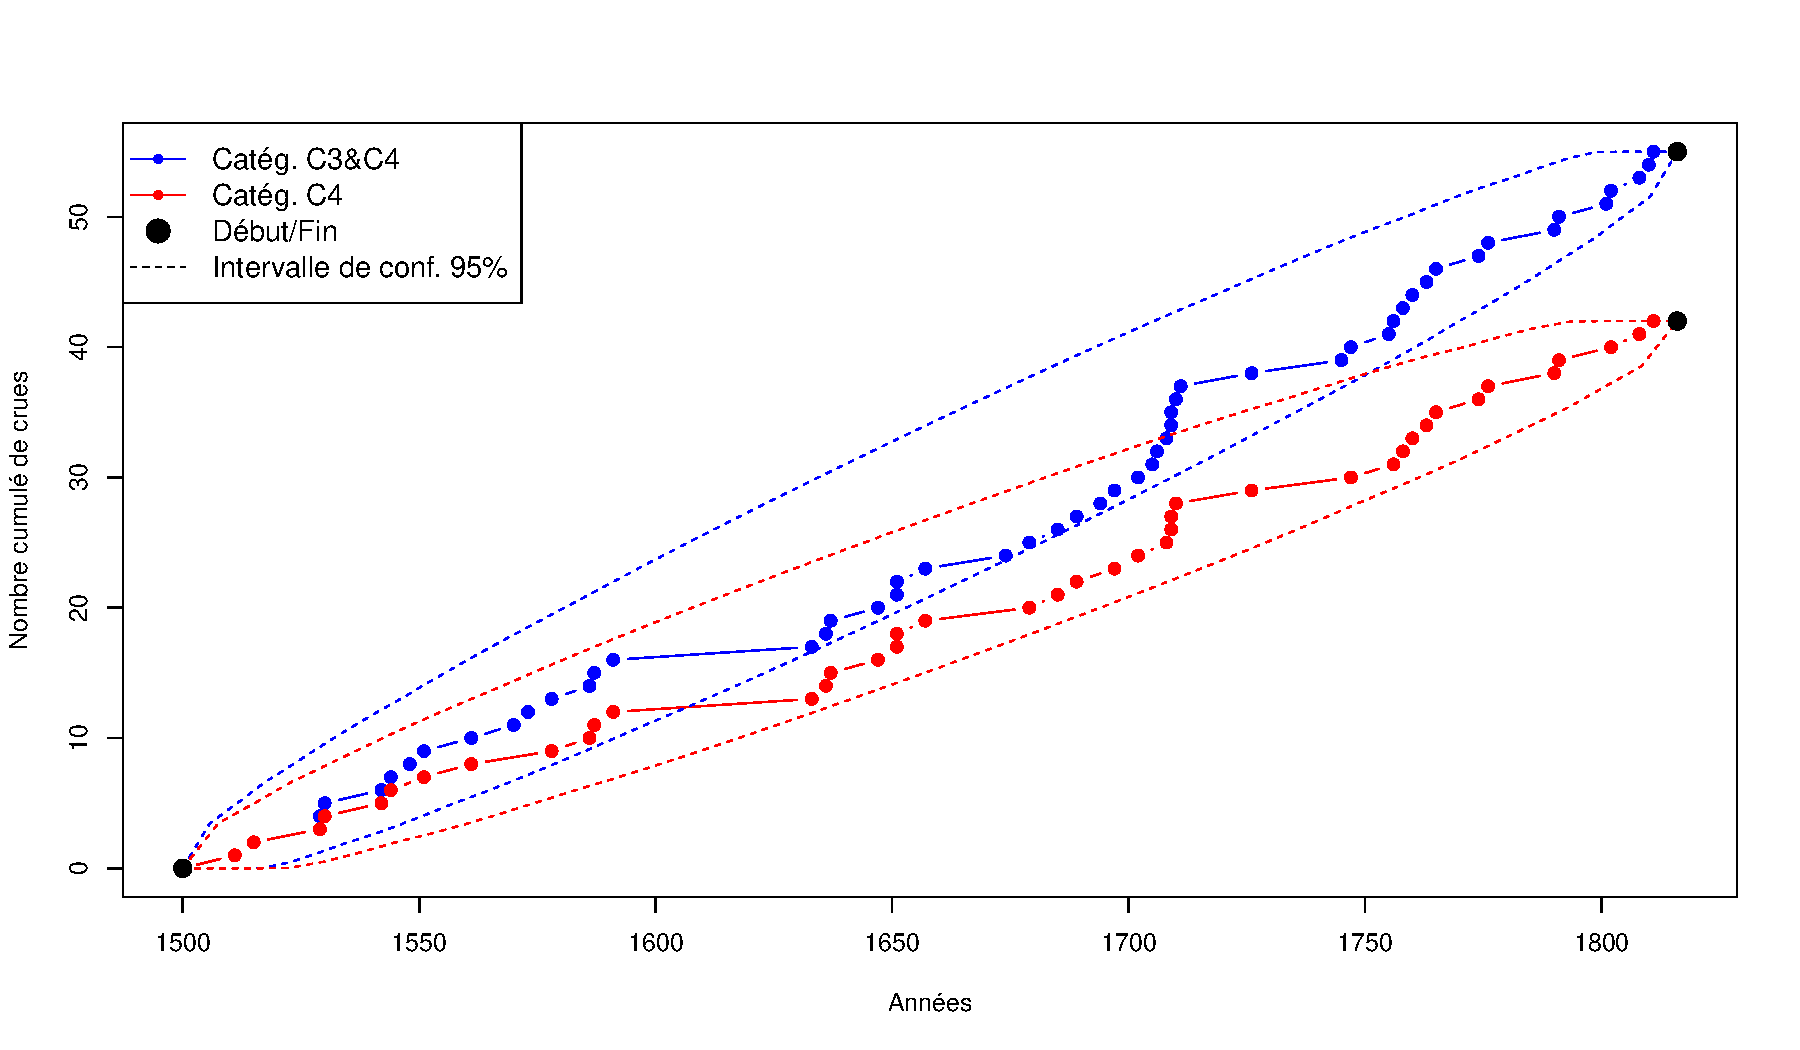
\includegraphics[width=.8\linewidth]{Figures/Poisson_C3-C4_FR.pdf}	
		\caption{Nombre de crues cumulé et intervalles de confiance à 95\% du processus de 						Poisson, pour deux échantillons d'occurrences de crues sup-seuil à Beaucaire 							(1500-1816)}
		\label{fig:Poisson_C3-C4}
	\end{figure}		
	
	\paragraph{} Sur la figure \ref{fig:Poisson_C3-C4}, on remarque que les nombre cumulés de crues des deux échantillons ne sortent pas des intervalles de confiance à 95\%, ils peuvent donc être tous deux considérés homogènes. L'échantillon correspondant au seuil $S3$ (en bleu) se rapproche de la borne inférieure de l'intervalle de confiance au XVII\textsuperscript{ème} siècle, mais revient rapidement dans des valeurs moyennes à la faveur de nombreuses crues sup-seuil au début du XVIII\textsuperscript{ème} siècle. 
	
	\paragraph{} L'échantillon continu de débits maximum annuels (1816-2020) sera par la suite artificiellement "dégradé" pour reproduire des durées de chroniques plus usuelles. Ainsi, les crues dont le débit maxpost est supérieur au seuil considéré sont retenues dans l'échantillon. Cette période "dégradée" commence au début de la chronique, en 1816, et se termine en 1970, à la mise en fonctionnement de la station de Beaucaire Restitution. Deux seuils de perception similaires aux seuils $S3$ et $S4$ sont ici étudiés : 7000 et 9000 $m^3/s$. L'homogénéité de ces deux échantillons "dégradés" est testée dans la figure \ref{fig:Poisson_Recent}. Les deux échantillons de crues cumulés ne sortent pas des intervalles de confiance à 95\%, ils sont donc tous deux homogènes. 
	
	\begin{figure}[h]
		\centering
		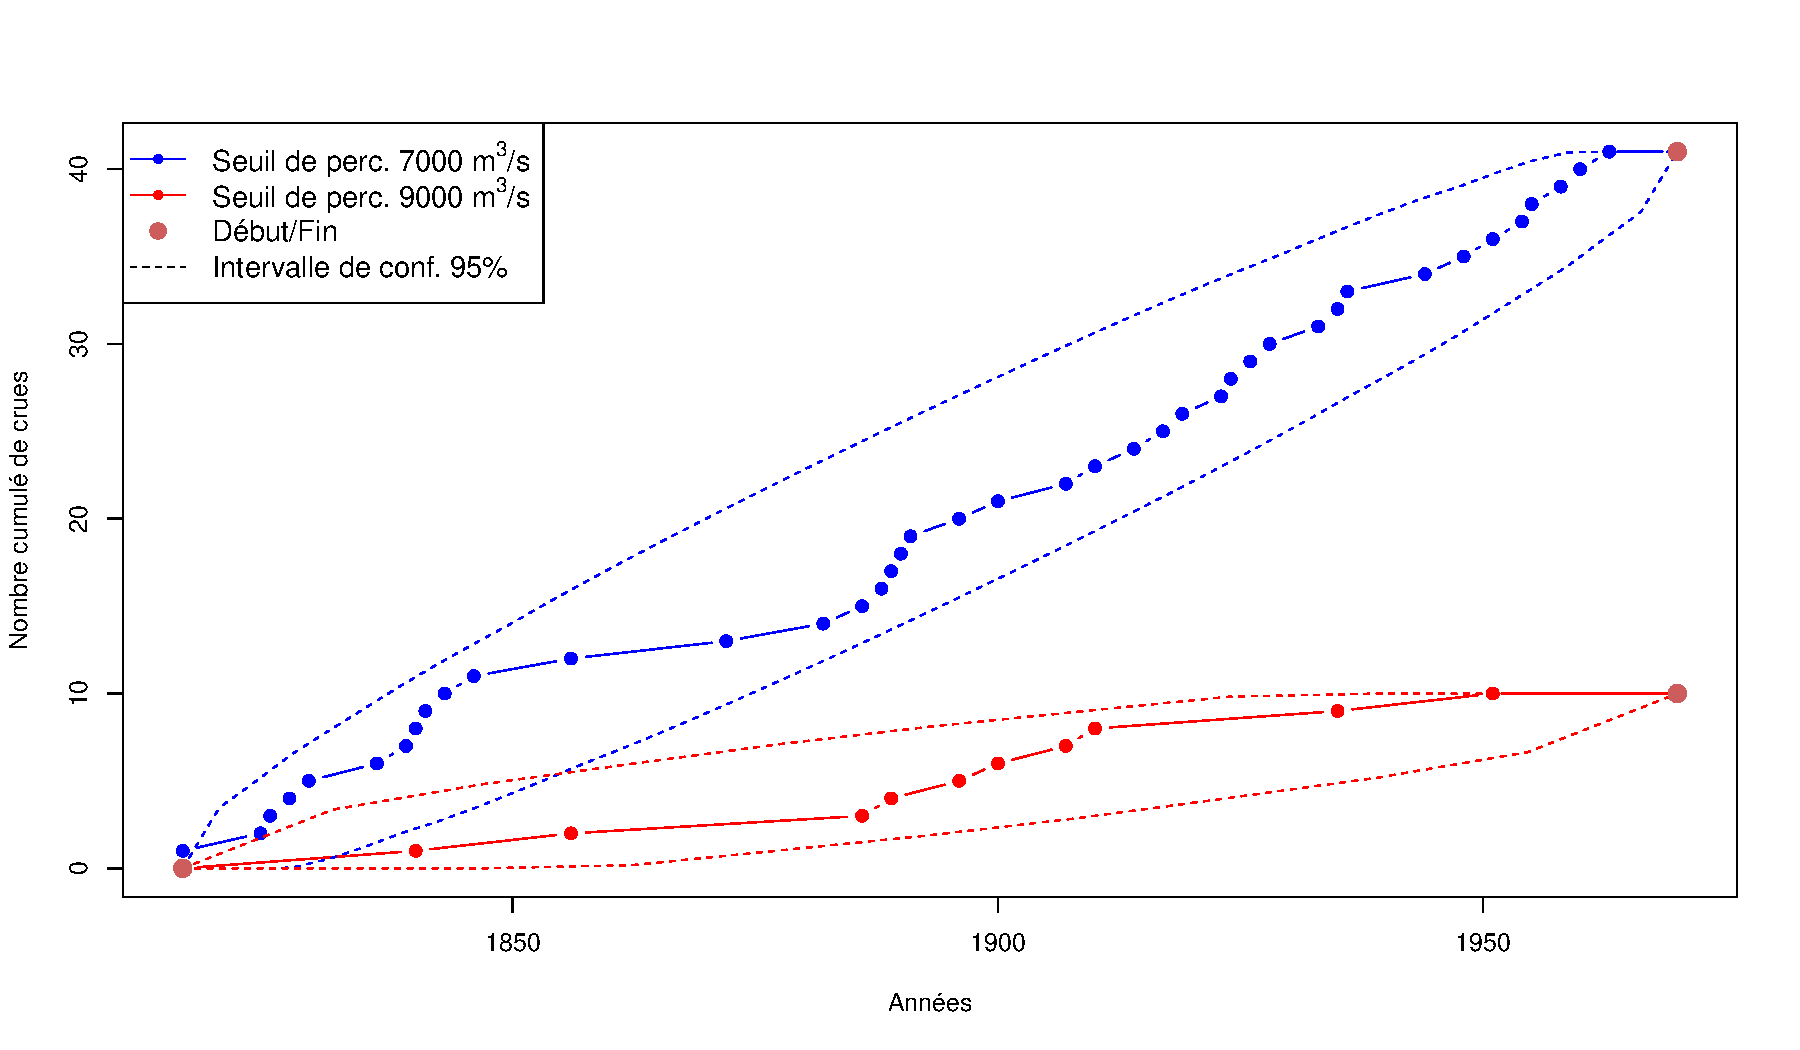
\includegraphics[width=.8\linewidth]{Figures/Poisson_Qrecent_FR.pdf}	
		\caption{Nombre de crues cumulé et intervalles de confiance à 95\% du processus de 						Poisson, pour deux échantillons d'occurrences de crues sup-seuil (S3 et S4) à Pont de Beaucaire 							(1816-1969) }
		\label{fig:Poisson_Recent}
	\end{figure}
	
	
		
\FloatBarrier		
	
	
\section{Application aux crues du Rhône à Beaucaire}

	\paragraph{}
	
	MICHEL : "Rappeler la signification avec une phrase/
Les quatre modèles décrits dans les sections précédentes :
* modèle A : incertitude uniquement sur les débits de la période continue. Pour la période historique, crues supérieures à un seuil connu et durée de la période historique connue;
* modèle B : pour la période historique, crues supérieures à un seuil incertain et durée de la période historique connue;
* modèle C : pour la période historique, crues supérieures à un seuil connu et durée de la période historique incertaine;
* modèle D : pour la période historique, crues supérieures à un seuil incertain et durée de la période historique incertaine;"

	Les 4 modèles décrits dans les sections précédentes (A, B, C et D) sont appliqués aux 4 échantillons de crues du Rhône à Beaucaire présentés dans le tableau \ref{tab:Echantillons}. Les échantillons 1 et 2 représentent la combinaison des données pré-1816 décrites dans le chapitre 2 REF avec les données continues 1816-2020 estimées au chapitre 1 (REF). Les échantillons 3 et 4 sont basés sur les débits estimés au chapitre 1(REF) qui ont été dégradés pour créer artificiellement un échantillon mixte de données continues (1970-2020) et ponctuelles (1816-1969). Il s'agit ici de tailles d'échantillon plus usuelles et dont le seuil de perception et la durée de la période historique sont parfaitement connus, contrairement aux échantillons 1 et 2. Ainsi, pour les modèles faisant l'hypothèse que le seuil de perception et/ou la durée de la période historique sont inconnus, on jugera notamment la capacité du modèle à converger vers des valeurs acceptables. 
	
% Please add the following required packages to your document preamble:
	\begin{table}[h]
		\centering
		\resizebox{\columnwidth}{!}{%
		%\begin{tabular}{|l|l|l|l|ll|l|l|}
		\begin{tabular}{|c|c|c|c|cc|c|c|}
		\hline
		\multicolumn{1}{|c|}{\multirow{2}{*}{n°}} &
		  \multirow{2}{*}{Période historique} &
		  \multirow{2}{*}{Période continue} &
		  \multirow{2}{*}{Seuil $S$ [m\textsuperscript{3}/s]} &
		  \multicolumn{2}{c|}{Nb. de crues $> S$} &
		  \multirow{2}{*}{A priori $S$ [m\textsuperscript{3}/s]} &
		  \multirow{2}{*}{A priori $t*$} \\ \cline{5-6}
		  
		 \multicolumn{1}{|c|}{} & & & & \multicolumn{1}{c|}{per. hist.} & per. cont. & & \\ \hline
		1 & 1500-1815 & 1816-2020 & 7000 & \multicolumn{1}{c|}{55} & 57 & $\mathcal{N}(7000,2000)$ & $\mathcal{U}(1111,1511)$ \\ \hline
		2 & 1500-1815 & 1816-2020 & 9000 & \multicolumn{1}{c|}{13} & 14 & $\mathcal{N}(9000,2000)$ & $\mathcal{U}(1129,1529)$ \\ \hline
		3 & 1816-1969 & 1970-2020 & 7000 & \multicolumn{1}{c|}{41} & 16 & $\mathcal{N}(7000,2000)$ & $\mathcal{U}(1316,1816)$ \\ \hline
		4 & 1816-1969 & 1970-2020 & 9000 & \multicolumn{1}{c|}{10} & 4 & $\mathcal{N}(9000,2000)$ & $\mathcal{U}(1340,1840)$ \\ \hline
		\end{tabular}%
		}
		\caption{Caractéristiques des échantillons de crues du Rhône à Beaucaire. REVOIR L'ORDRE DES LIGNES}
		\label{tab:Echantillons}
	\end{table}		
	
	
	MICHEL : "EXPLIQUER CHOIX sigma =  2000 m3/s  pour incertitude S, et longueur intervalle loi uniforme = 400 ans pour date début période historique.

Expliquer : 1511 année première crue catégorie C3  sur 1500-1815 ; 1529 année première crue catégorie C4  sur 1500-1815 ; 1816 année première crue catégorie C3  sur 1816-1969 ; 1840 année première crue catégorie C4  sur 1816-1969

	
	Pour les modèles qui font l'hypothèse d'un seuil de perception connu (A et C), le seuil retenu est présenté dans le tableau \ref{tab:Echantillons}. Il en est de même pour les modèles qui font l'hypothèse d'une durée de période historique connue (B et D). Ici, par souci de clarté, ce n'est pas la durée de la période historique $n$ qui sera examinée mais la date de début de la période historique $t*$. Lorsque cette date est supposée méconnue, l'a priori débute à la date de la première crue de l'échantillon.
			
	\FloatBarrier	
	
	\subsection{Résultats pour la période récente dégradée (1816-2020)}
	
	\paragraph{} 
	Les 4 modèles décrits dans la section (REF) ont été appliqués à l'échantillon 4 du tableau \ref{tab:Echantillons}. Les estimations pour les crues centennales et millénales sont présentés dans la figure \ref{fig:Barplot_Artif2}, dans laquelle les 4 modèles GEV-Binomiale sont comparés au modèles GEV (chapitre 1 (REF)) pour la chronique continue totale (1816-2020) et la chronique continue dégradée (1970-2020). 
	
	\begin{figure}[h]
		\centering
		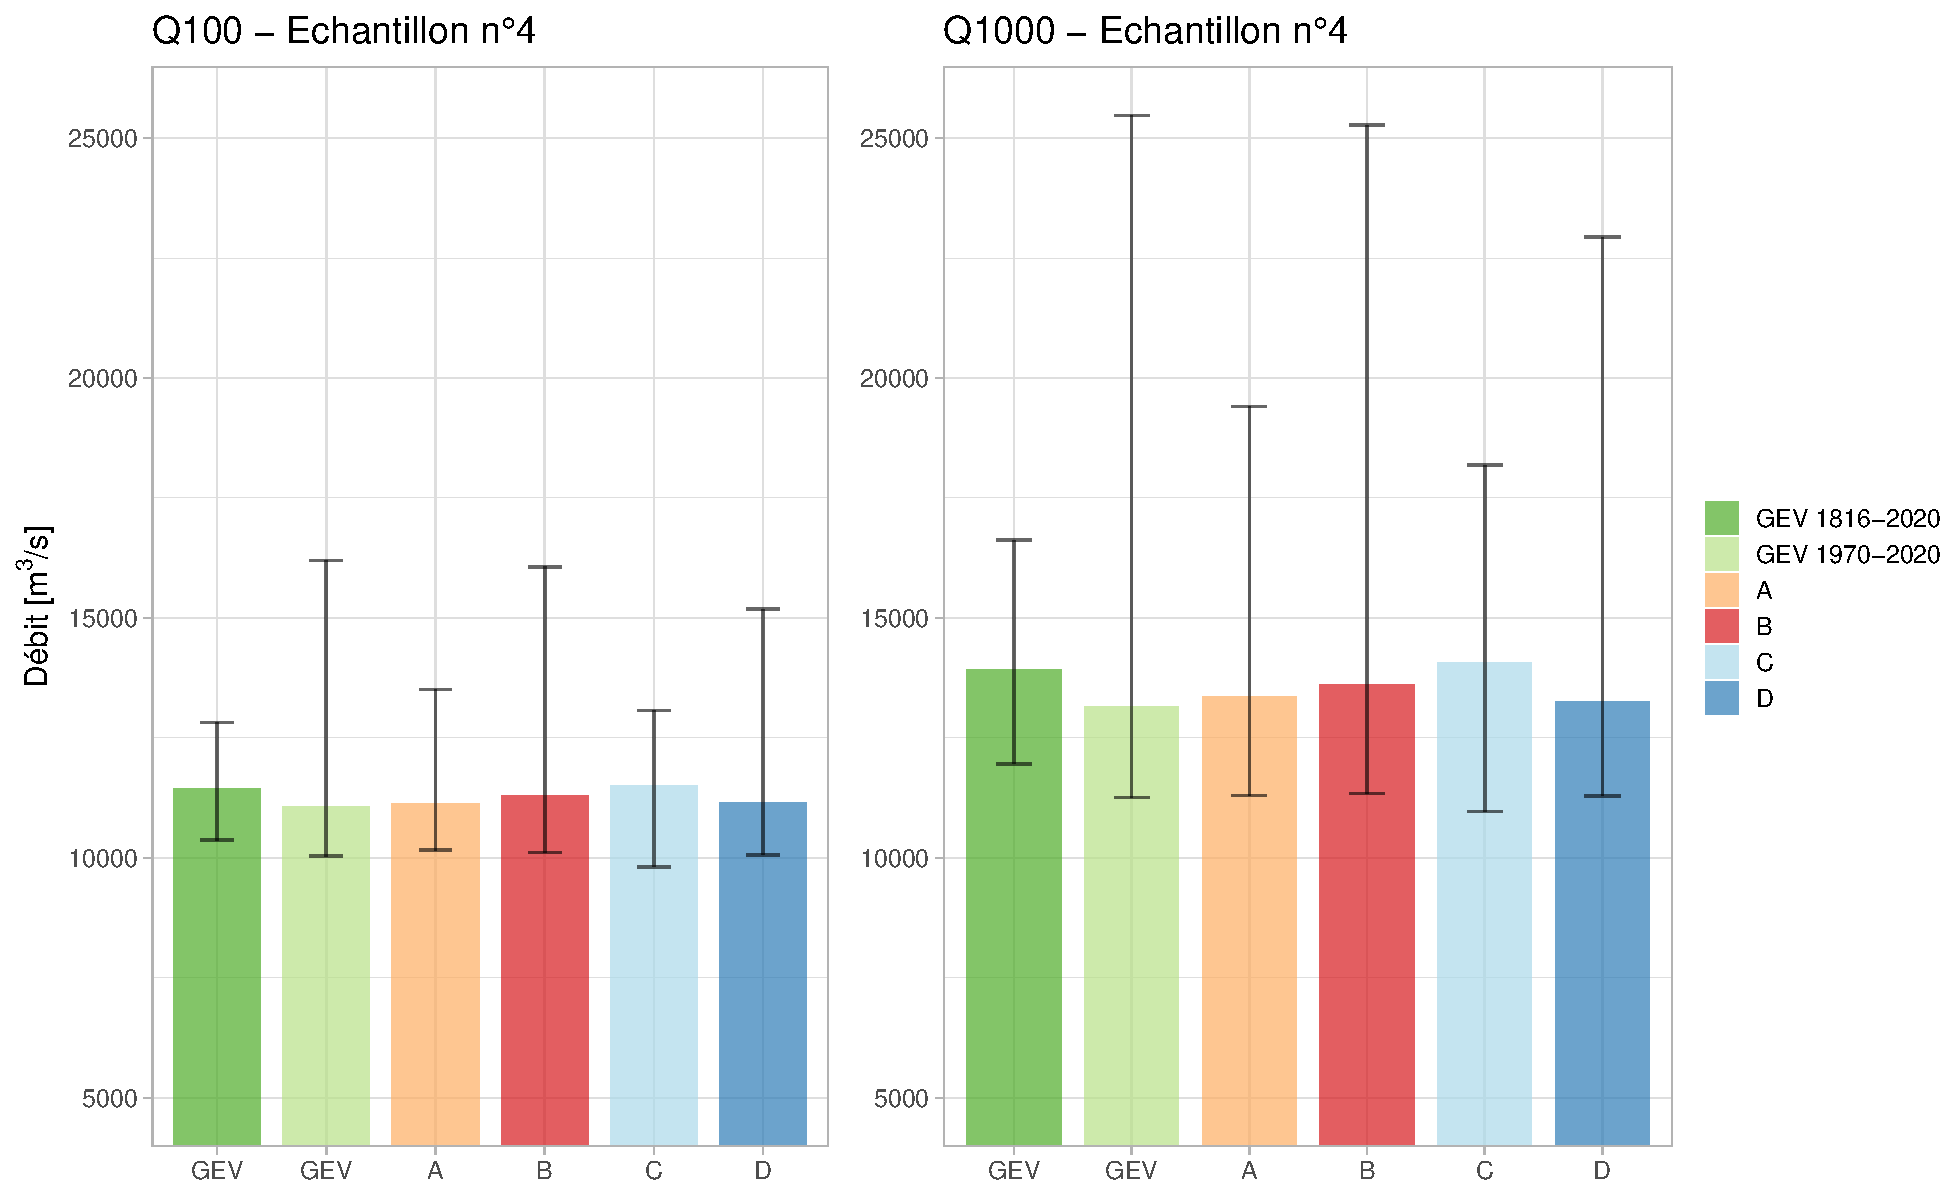
\includegraphics[width=.8\linewidth]{Figures/Barplots_QX_Artif2.pdf}	
		\caption{Estimations maxpost et incertitudes à 95\% pour Q100 et Q1000 par 6 modèles différents pour l'échantillon 4 (1816-2020 dégradé, $S4$)}
		\label{fig:Barplot_Artif2}
	\end{figure}
	
	\paragraph{} On observe tout d'abord dans la figure \ref{fig:Barplot_Artif2} que l'incertitude du modèle GEV pour la période 1970-2020 est la plus importante de tous les modèles (VALEUR EN \% ?). Cinquante années de données continues ne permettent pas d'obtenir une précision acceptable. Cela souligne l'intérêt de valoriser les données historiques dans une situation de ce type. Globalement, les estimations maxpost de l'ensemble des modèles sont proches. En revanche, les enveloppes d'incertitude sont très variables d'un modèle à l'autre, tout particulièrement pour les estimations millénales. 	
	
	\begin{figure}[h]
		\centering
		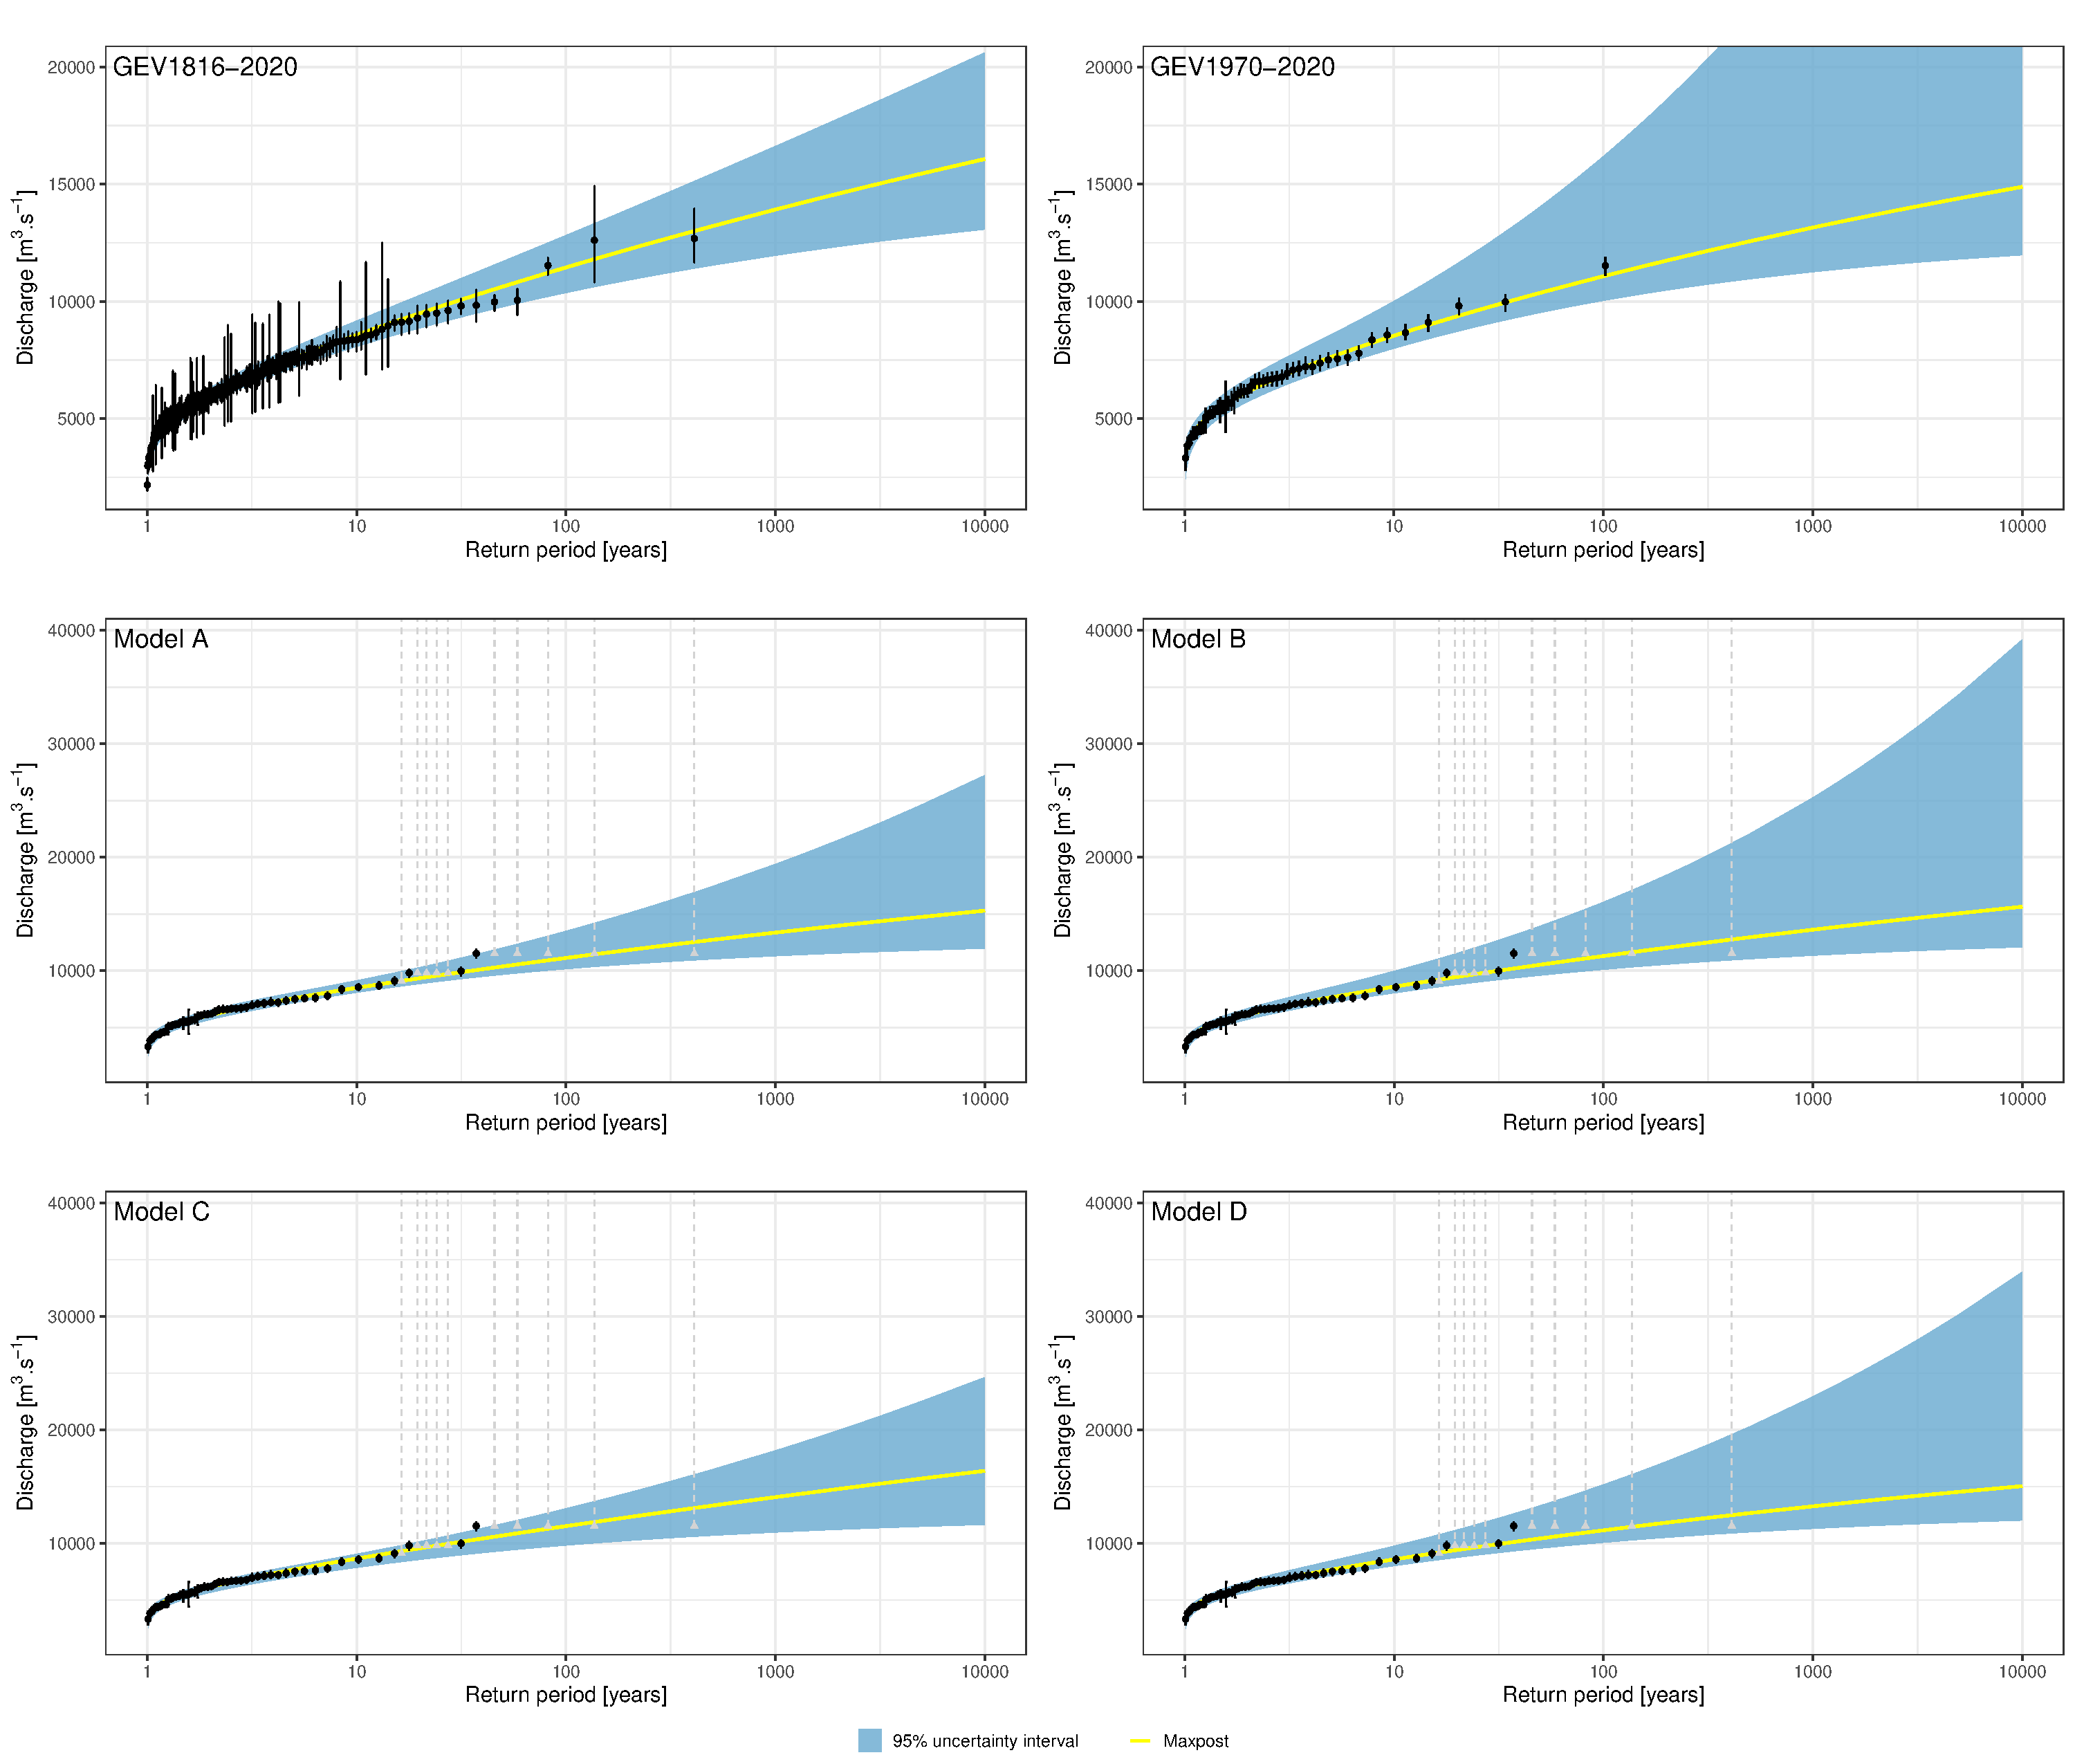
\includegraphics[width=\linewidth]{Figures/Quantiles_Artif2.pdf}	
		\caption{Quantiles de débit maximum annuel estimés par 6 modèles pour l'échantillon 4 (1816-2020 dégradé, $S4$). Les observations sont en noir pour la période continue et en gris pour la période historique.}
		\label{fig:Quantiles_Artif2}
	\end{figure}
	
	\paragraph{} La figure \ref{fig:Quantiles_Artif2} présente l'ensemble des quantiles jusqu'à la crue décamillénale pour les 6 modèles. Ici, le rang des crues sup-seuil des deux périodes a été tiré aléatoirement comme décrit dans la section (REF). Les estimations sont cohérentes avec les observations pour les 6 modèles. On remarque que l'incertitude croît rapidement au-delà la crue centennale pour les modèles B, D et GEV 1970-2020. 

\FloatBarrier
	
	\subsubsection{Quel est l'apport de l'utilisation des crues historiques pour une longueur de chronique "courante" ?}
	
	\paragraph{} Une durée de chronique continue trop courte devant le quantile visé entraîne des résultats très incertains (GEV 1970-2020 en vert clair sur la figure \ref{fig:Barplot_Artif2}). Ici, la durée de la chronique continue de 50 ans est très petite devant la période de retour visée de 100 ou 1000 ans. Si on se trouve dans l'impossibilité de reconstituer des débits en continu au-delà de 50 ans, on remarque que l'utilisation d'occurrences de crues historiques permet de réduire l'incertitude (modèle A en orange). Évidemment, l'utilisation de témoignages de crues ne permet pas d'atteindre la précision obtenue avec 200 ans de chronique continue (GEV 1816-2020 en vert foncé), mais l'incertitude obtenue s'en rapproche. Une part de cette incertitude pour l'ensemble des modèles provient notamment de l'estimation du paramètre de forme, qui gouverne le comportement de la queue de distribution. On retrouve les valeurs a posteriori du paramètre de forme dans la figure \ref{fig:Shape_Artif2}. On notera que l'ensemble des estimations sont proches de zéro et légèrement positives, on se trouve donc dans le cas "queue légère" de la distribution GEV. On remarque que l'estimation de ce paramètre est plus précise dans le cas GEV 1816-2020 que dans tous les autres cas. Dans le cas du modèle A, l'estimation du paramètre de forme est similaire à celle du modèle GEV pour l'échantillon 1970-2020. En effet, seuls les paramètres de la distribution GEV sont estimés par le modèle A, le seuil de perception et la durée de la période historique étant supposés précisément connus, ce qui n'est pas toujours le cas. 
	
	\begin{figure}[h]
		\centering
		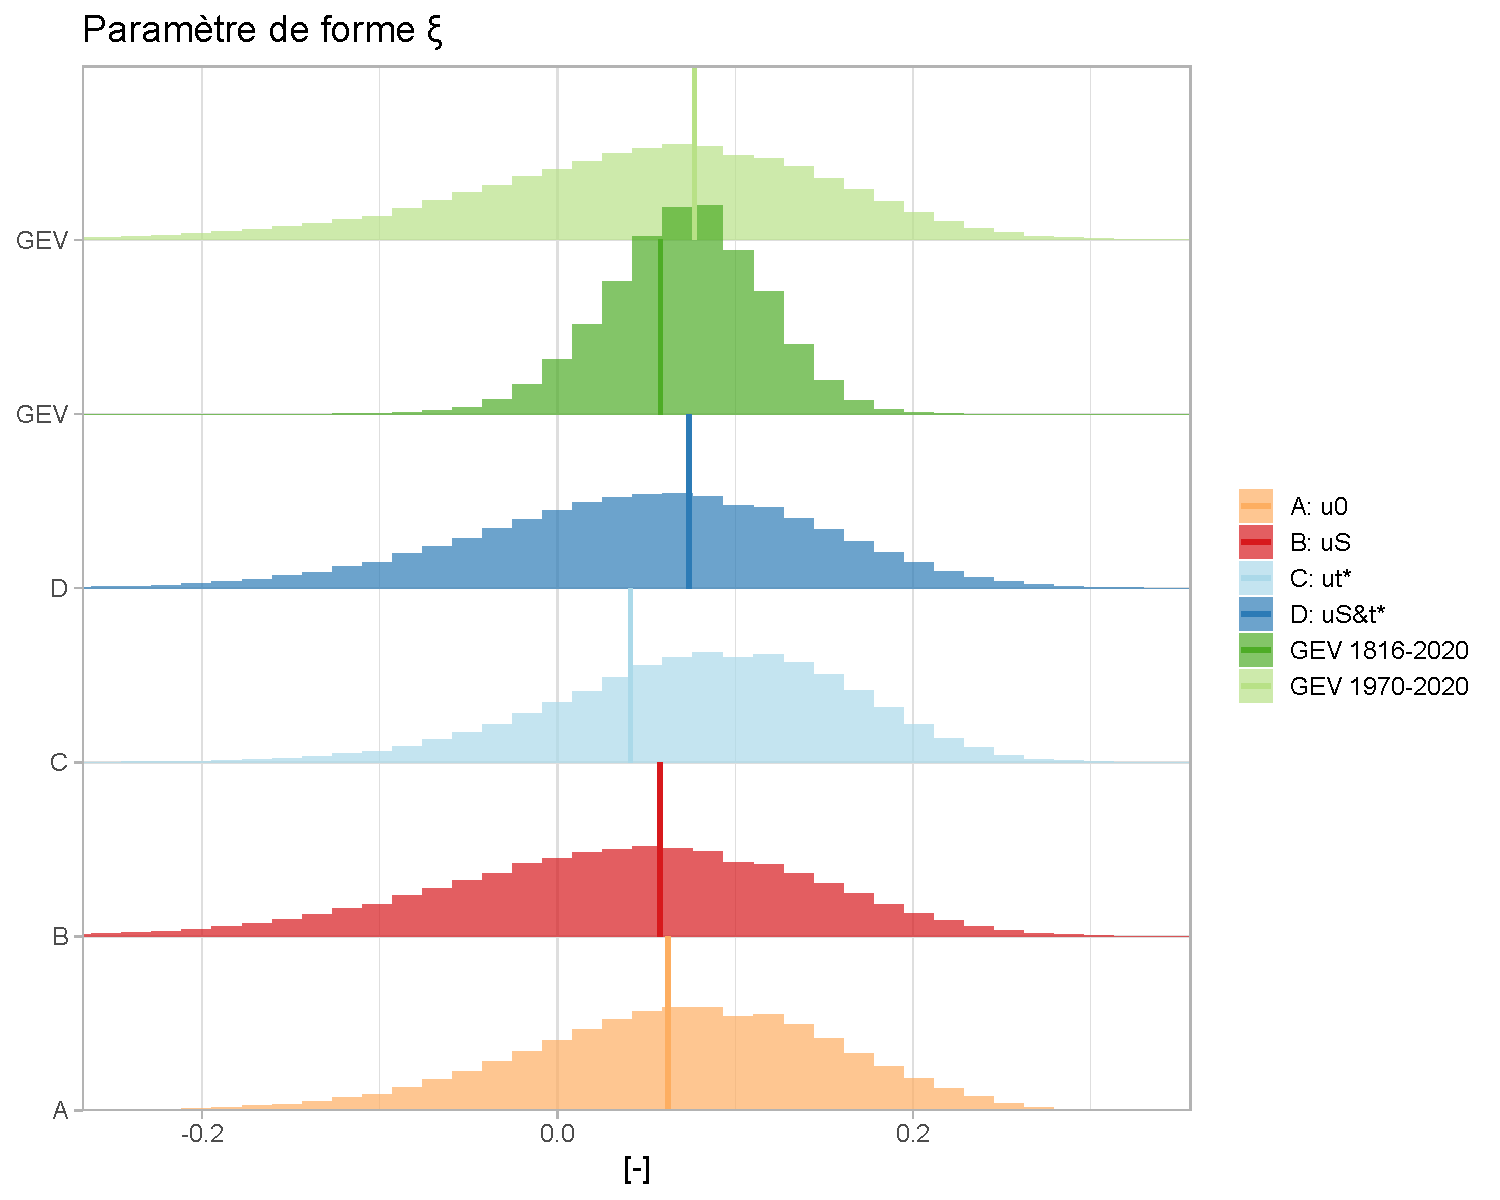
\includegraphics[width=.6\linewidth]{Figures/Shape_Artif2.pdf}	
		\caption{Distributions a posteriori du paramètre de forme de la distribution GEV des débits maximum annuels pour les 4 modèles estimés sur l'échantillon 4. Les estimations des modèles GEV sont également indiquées. Les droites verticales représentent les valeurs maxpost.}
		\label{fig:Shape_Artif2}
	\end{figure}

\FloatBarrier
	
	\subsubsection{Quel est l'impact de la méconnaissance du seuil de perception sur l'estimation des quantiles ?}
	
	\paragraph{} L'utilisation du modèle B reflète la méconnaissance du seuil de perception, celui-ci devenant alors un paramètre à part entière du modèle. Sur la figure \ref{fig:Barplot_Artif2}, on constate que l'incertitude autour des quantiles estimés par le modèle B est bien plus importante que pour le modèle A. La méconnaissance du seuil a donc des conséquences importantes sur les estimations. La vraie valeur du seuil de perception pour l'échantillon 4 est $S4$ = 9000 m\textsuperscript{3}/s. On retrouve les distributions a priori et a posteriori du seuil dans la figure \ref{fig:Params_Artif2}. On remarque que l'a posteriori (VALEUR) pour le modèle B est proche de la vraie valeur et que le modèle a effectivement permis d'améliorer la connaissance du seuil par rapport à l'a priori renseigné qui est ici très large : $\mathcal{N}(9000,2000)$. La valeur maxpost est de 9163 m\textsuperscript{3}/s soit une erreur relative de 2\% (ECART TYPE). Néanmoins, une telle méconnaissance de ce paramètre impacte grandement l'estimation des quantiles. Dans une situation plus réaliste, un a priori plus précis aurait pu être choisi afin de limiter cet impact. 
	
	 \begin{figure}[h]
		\centering
		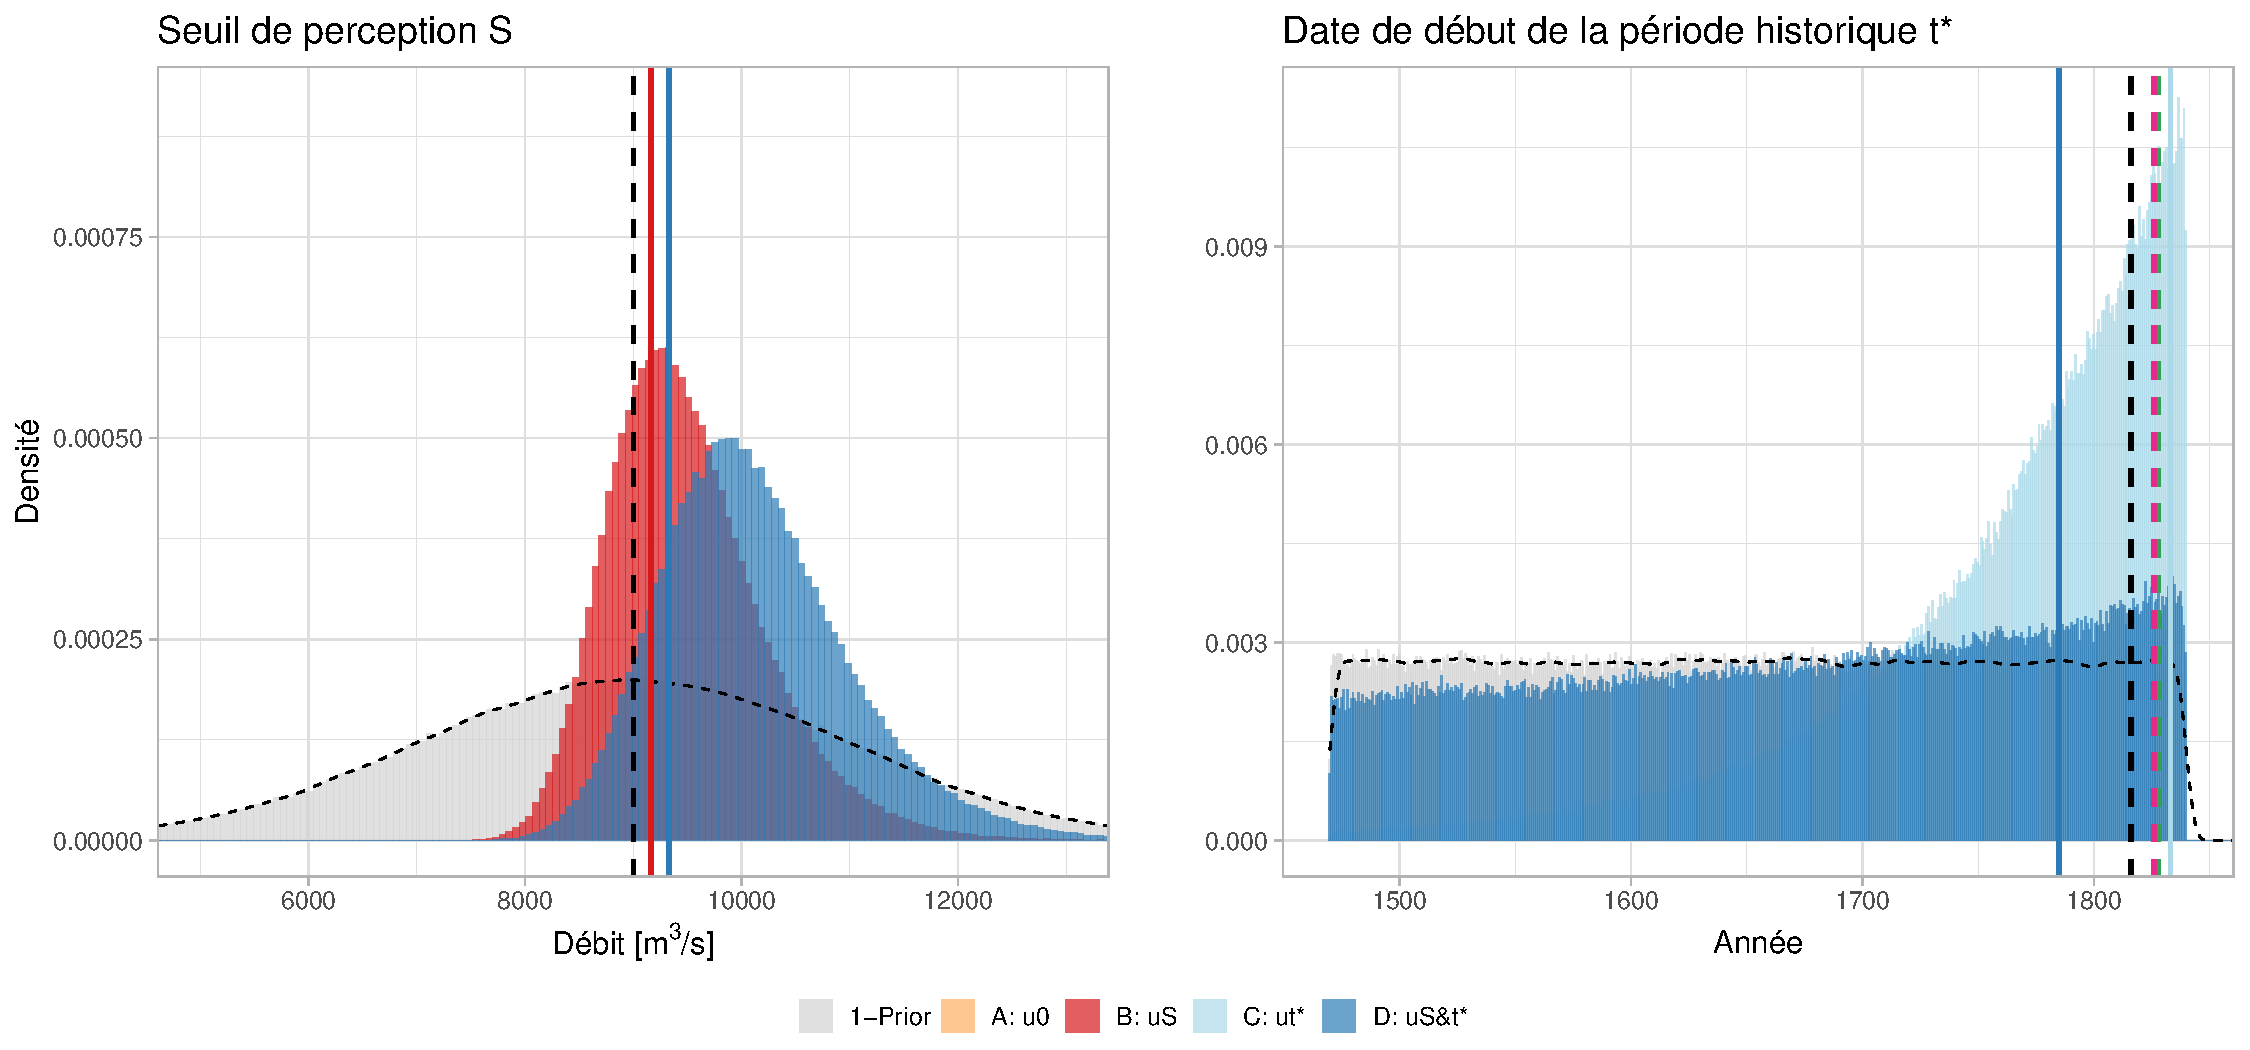
\includegraphics[width=.9\linewidth]{Figures/Params_Artif2.pdf}	
		\caption{Distributions a priori et a posteriori pour le seuil de perception (gauche) et la date de début de la période historique (droite). Les droites verticales pleines représentent l'estimation maxpost du paramètre pour chacun des modèles. La droite verticale noire en pointillés représente à gauche le vrai seuil de perception ($S4$ = 9000 m\textsuperscript{3}/s), et à droite la vraie date de début de la période historique ($t*$ = 1816). Les droites verticales en pointillés vert et rose représentent respectivement les estimations de $t*$ par les méthodes \cite{prosdocimi_german_2018} et de la période de retour du seuil $S$.}
		\label{fig:Params_Artif2}
	\end{figure}
	
	\subsubsection{Quel est l'impact de la méconnaissance de la durée de la période historique sur l'estimation des quantiles ?}	
	
	\paragraph{} Le modèle C permet de représenter la méconnaissance de la durée de la période historique, qui est l'un des deux paramètres de la loi binomiale utilisée ici pour modéliser le nombre d'occurrences de crues sup-seuil. Sur la figure \ref{fig:Barplot_Artif2}, les estimations maxpost des quantiles pour le modèle C ont des valeurs légèrement supérieures aux estimations du modèle A. Cette légère sur-estimation provient d'une durée de période historique sous-estimée par le modèle, visible sur la figure \ref{fig:Params_Artif2} (droite). En effet, la date maxpost est l'année 1833, alors que la chronique débute réellement en 1816. Cette sur-estimation peut s'expliquer par une fréquence des crues sup-seuil plus importante au cours de la période continue (4 crues / 50 ans = 0.08 crues/an) qu'au cours de la période historique (10 crues / 153 ans = 0.065 crues/an). Ce déséquilibre reflète l'existence de phases durant lesquelles la fréquence d'occurrence des crues sup-seuil oscille malgré le fait qu'aucune non-stationnarité des données n'ait été détectée par les tests à la section (REF). L'impact de ces phases est exacerbé par des longueurs de chronique trop petites devant la durée de ces oscillations. 
	\paragraph{} L'incertitude autour des quantiles estimée par le modèle C est très similaire à celle estimée par le modèle A (figure \ref{fig:Barplot_Artif2}), de même que la distribution du paramètre de forme (figure \ref{fig:Shape_Artif2}), et ce malgré un a priori très peu informatif pour la date de début de la période historique : ($\mathcal{U}(1340,1840)$). Une forte méconnaissance de la durée de la période historique n'a donc que peu d'impact sur la précision de l'estimation des quantiles, contrairement à la méconnaissance du seuil de perception.
	
	\subsubsection{Quel est l'impact de la méconnaissance du seuil de perception et de la durée de la période historique sur l'estimation des quantiles ?}	
	
	\paragraph{} Représenter la méconnaissance de ces deux données en même temps paraît être la solution la plus raisonnable dans le cas d'événements très anciens et pouvant être peu précisément décrits dans les témoignages. Le modèle D est ici utilisé à cet effet. Les quantiles maxpost estimés dans la figure \ref{fig:Barplot_Artif2} pour le modèle D semblent cohérents avec les valeurs de référence. En revanche, la largeur de l'intervalle de confiance est importante et se situe entre celle du modèle B et du modèle C. Même si l'estimation est plus précise que celle du modèle GEV sur l'échantillon 1970-2020, elle reste imprécise pour la crue millénale. L'observation des paramètres a posteriori sur la figure \ref{fig:Params_Artif2} permet de comprendre l'origine de cette large incertitude. La distribution du seuil de perception, bien que centrée a proximité de la vraie valeur (maxpost à 9331 $m^3/s$), est très large : VALEUR ECART TYPE. Le seuil de perception parait ici un peu moins bien estimé que par le modèle B. La date de début de la période historique est elle encore plus difficilement estimée. On remarque que la distribution a posteriori est pratiquement aussi large que celle de l'a priori, même si elle marque un maximum non loin de la vraie valeur (l'année 1816). La plus faible incertitude autour des quantiles pour le modèle D par rapport au modèle B provient de corrélations entre les paramètres qui peut être observée sur la figure \ref{fig:ScatterD_Artif2}. On remarque notamment une assez bonne corrélation entre la durée de la période historique et le seuil de perception, ainsi qu'entre le seuil de perception et le paramètre de forme. Il est donc complexe d'identifier ces paramètres séparément. Une élicitation plus précise de leurs a priori est ici nécessaire 
	
	\begin{figure}[h]
		\centering
		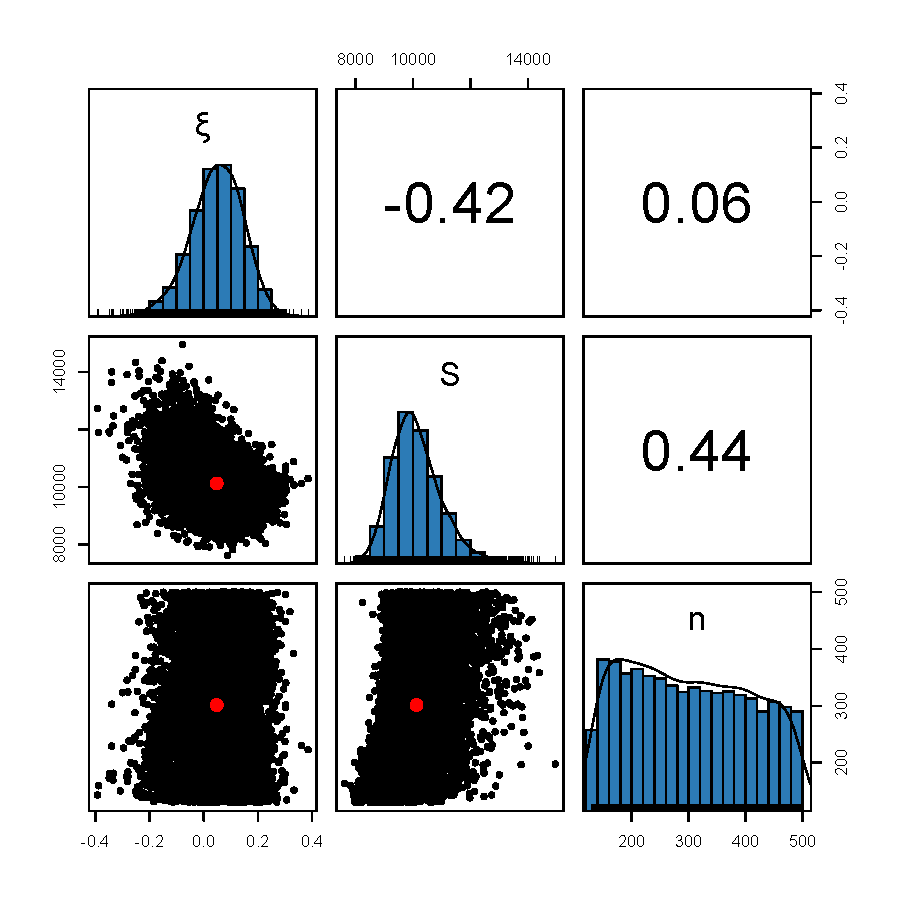
\includegraphics[width=.7\linewidth]{Figures/ScatterD_Artif2.pdf}
		\caption{Scatterplot des distributions a posteriori de trois paramètres du modèle D pour l'échantillon 4 : le paramètre de forme $\xi$ (sans unité), le seuil de perception $S$ (en $m^3/s$) et la durée de la période historique $n$ (en années). Les nombres inscrits dans les cases supérieures correspondent aux corrélations entre les paramètres.}
		\label{fig:ScatterD_Artif2}
	\end{figure}
	
%	\paragraph{} Les paramètres a posteriori sont présentés dans la figure \ref{subfig:Params_Artif2}. Les paramètres de forme estimés sont tous proches de la référence, soit légèrement positifs. Pour le seuil de perception dont la vraie valeur est ici 9000 $m^3/s$, les estimations maxpost pour les modèles B et D sont respectivement de 9163 et 9331 $m^3/s$. Le modèle converge donc vers des valeurs très proches. En revanche, la distribution pour le modèle D semble décalée vers des valeurs plus fortes, probablement pour compenser l'estimation d'une durée de période historique trop longue. Sur le graphique de droite, la durée de la période historique est présentée sous la forme de la date de début de la période dont la vraie valeur est ici est l'année 1816. L'a  priori étant une distribution uniforme qui débute à l'année de la première crue de l'échantillon (ici en 1840), il est possible de trouver des dates plus anciennes ou plus récentes que la vraie valeur. La période historique estimée par le modèle C débute en 1833, elle est donc plus courte que la réalité. En revanche, le modèle D estime un début de période maxpost en 1785. La distribution des durées de période du modèle C semble bien plus raisonnable que celle du modèle D, pour lequel la densité est pratiquement uniforme et donc très proche de l'a priori (qui pour cette raison n'est pas visible ici). Sans surprise, une méconnaissance du seuil et de la durée de la période historique complexifie l'estimation des paramètres. Quand un seul des deux est méconnu, les paramètres sont en revanche bien mieux estimés. Il faut aussi noter que ces résultats sont dépendants du choix du seuil de perception "artificiel", fixé ici à 9000 $m^3/s$ (il est dépassé par 10 crues entre 1816 et 1970).
%	\\
%	Les résultats pourraient être différents pour un autre seuil, monter A artif1 VS A artif 2? \\
%	(AJOUTER LE SCATTERPLOT POUR LE MODELE D?)\\
%	(GRAPHE DES QUANTILES?)\\
	
%	\begin{figure}[h]
%        \centering
%        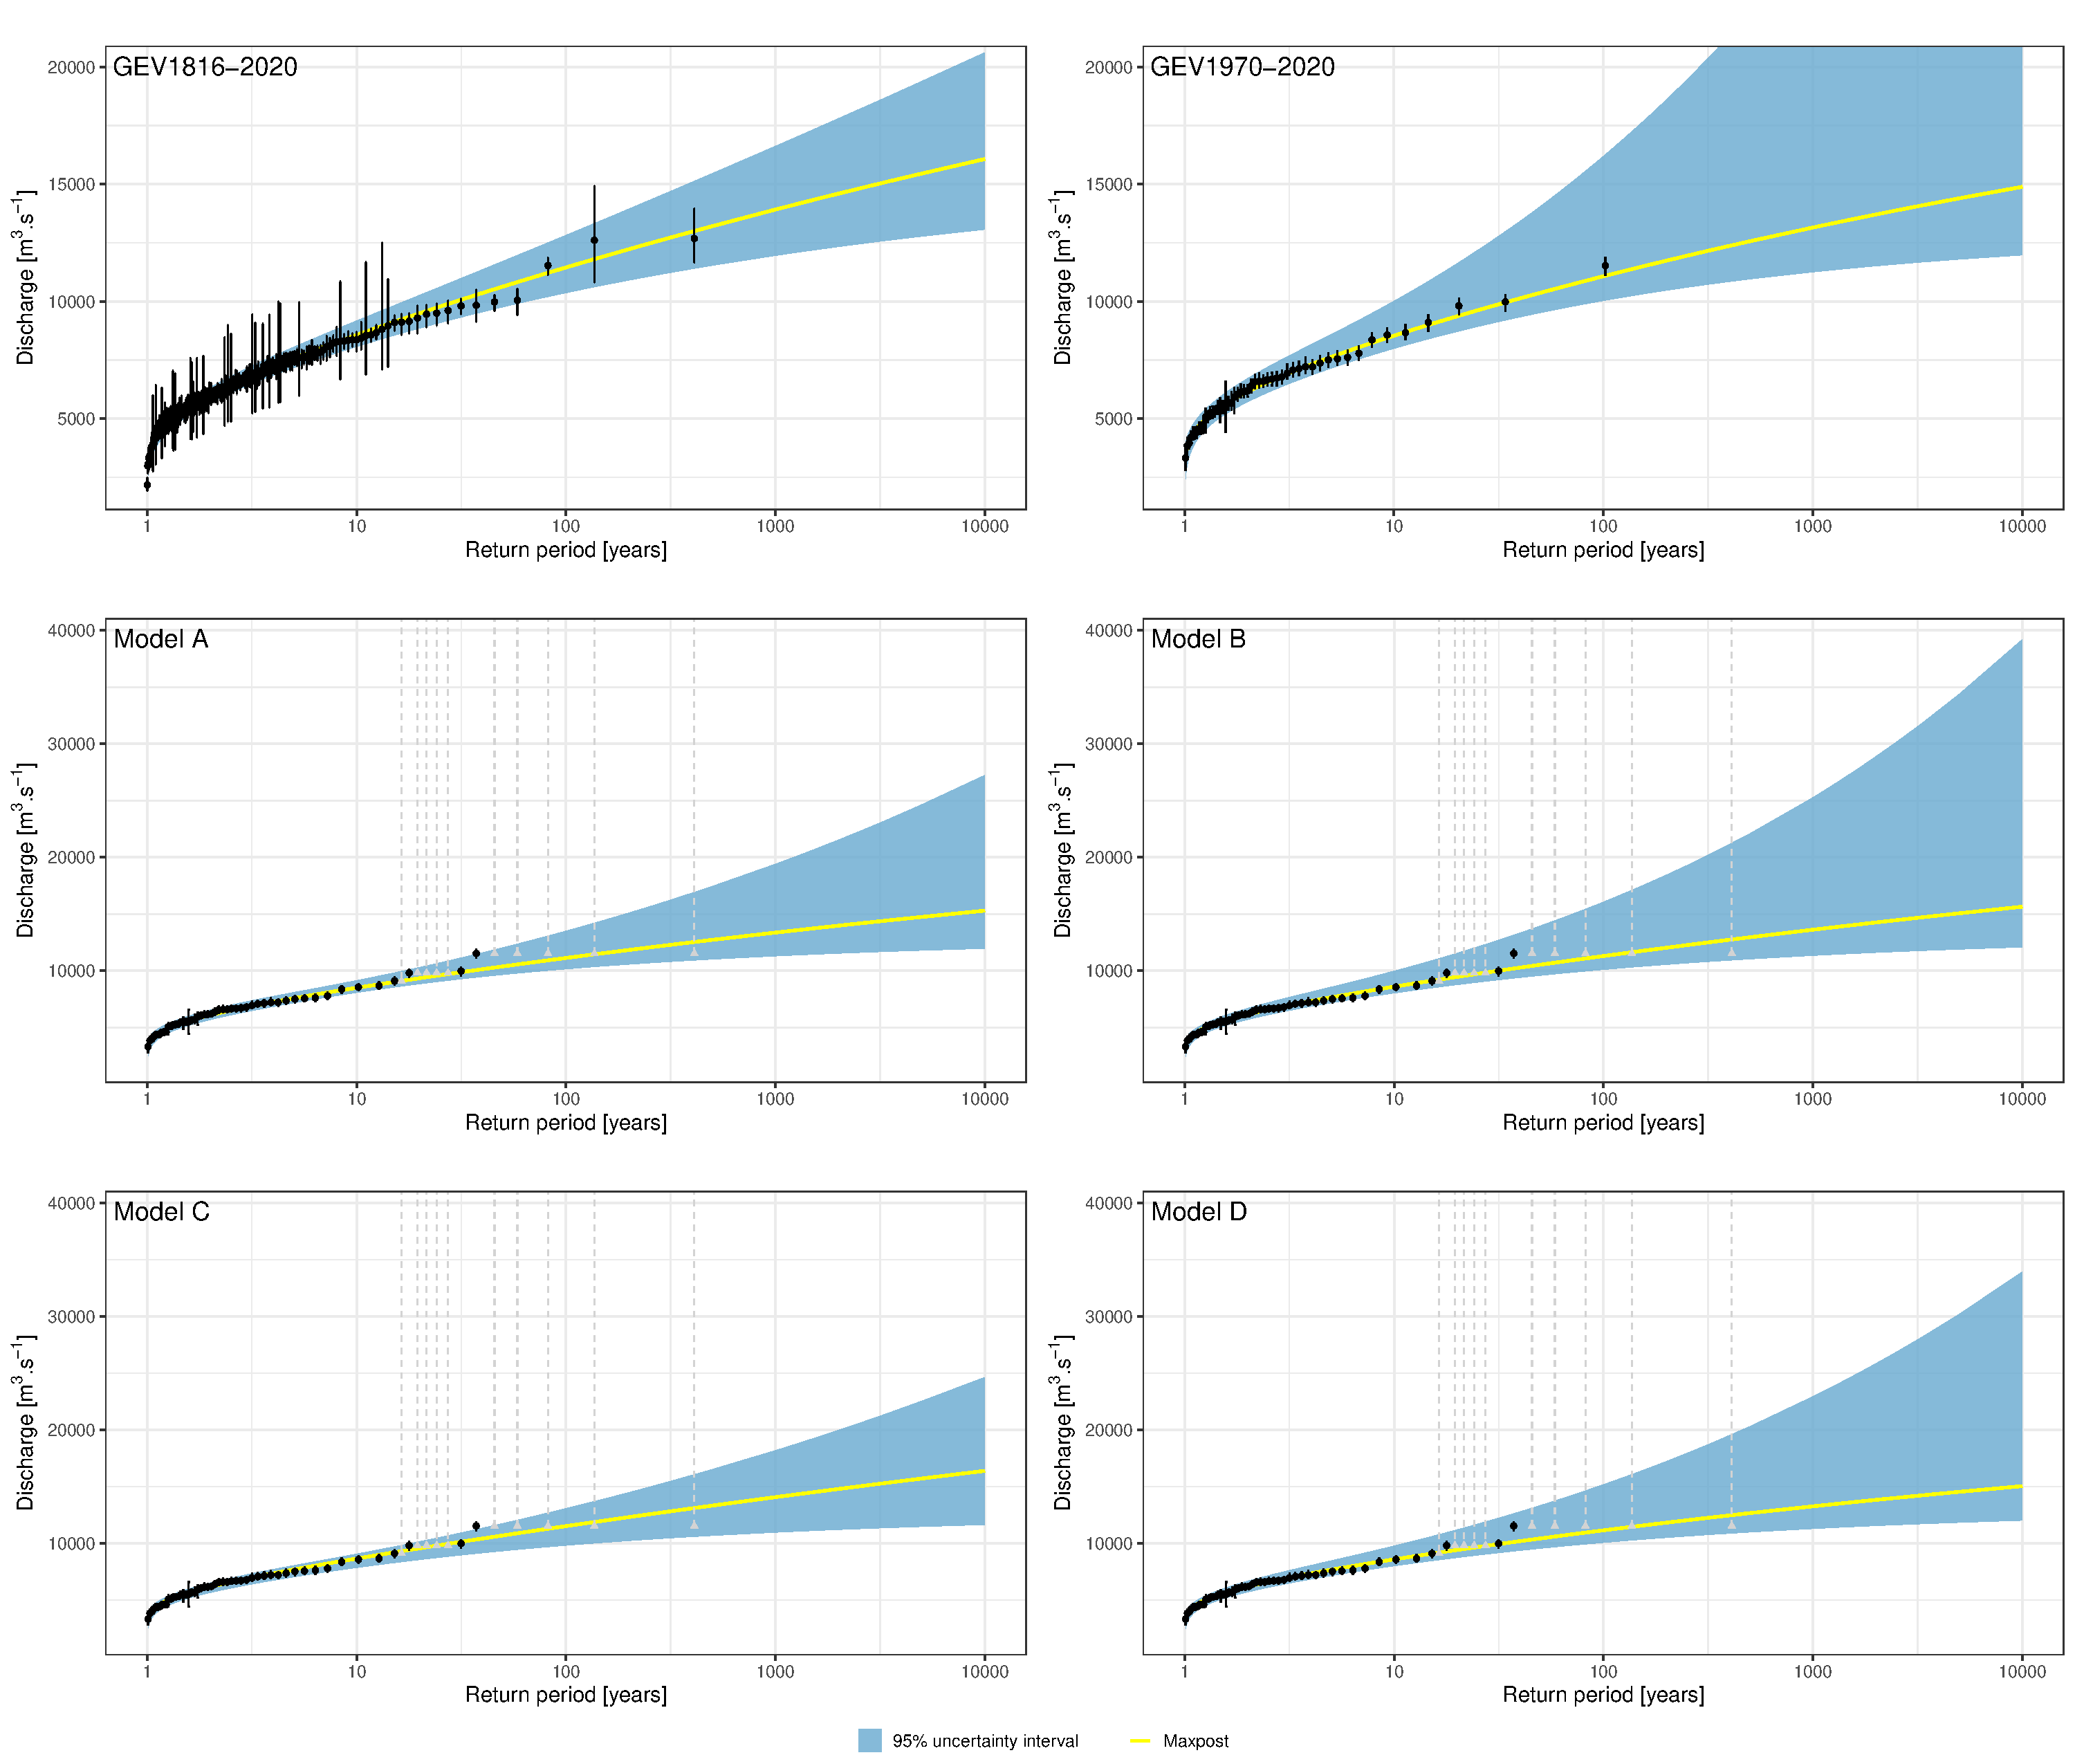
\includegraphics[width=.9\linewidth]{Figures/Quantiles_Artif2.pdf}
%        \caption{Quantiles estimés sur l'échantillon 2 pour les 6 modèles. Les crues de la période continue sont en noir, les crues de la période historiques en gris}
%        \label{fig:Quants_Artif2}
%%\end{figure}
		
\FloatBarrier

	\subsubsection{Quel est l'apport de la connaissance du débit des crues historiques ?}


	\begin{figure}[h]
		\centering
		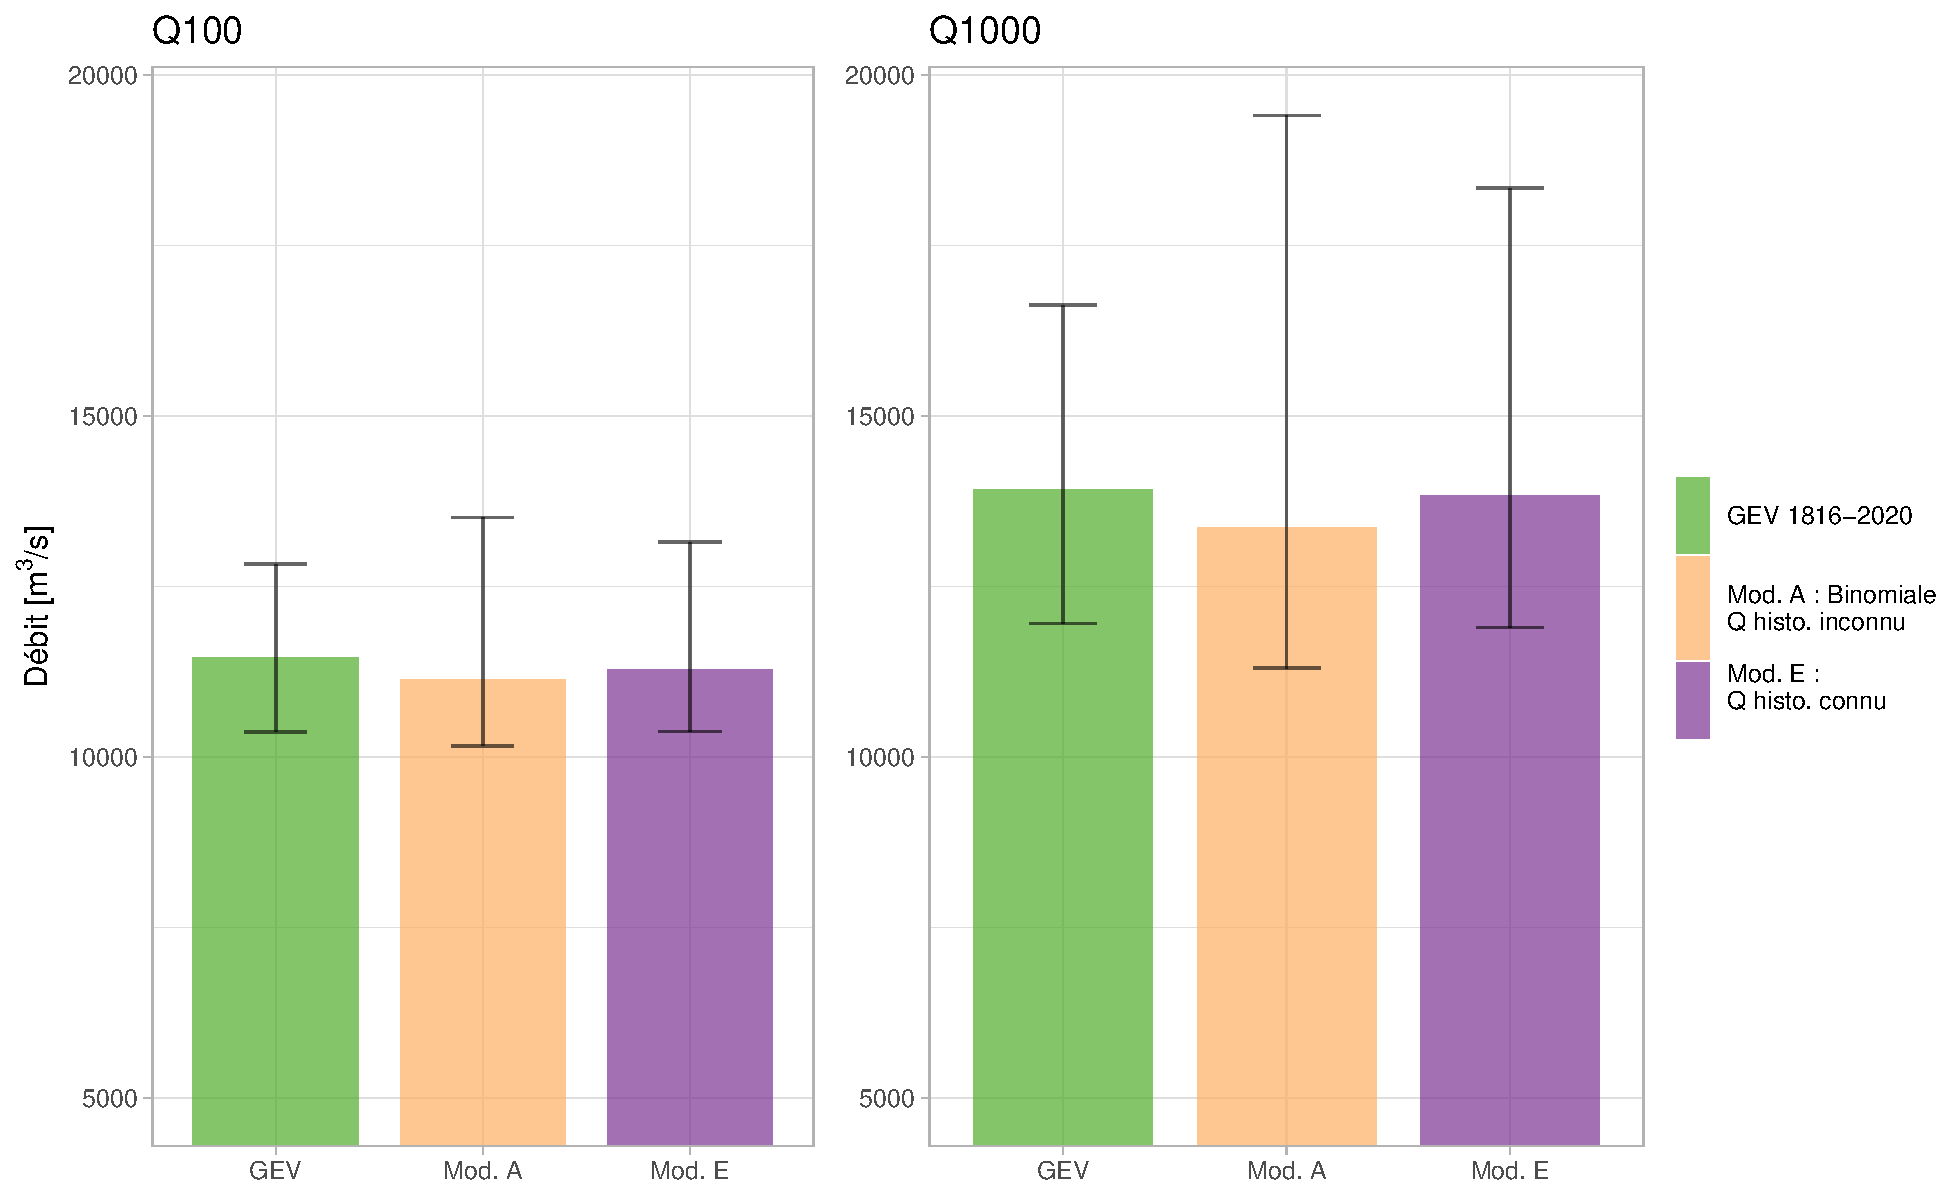
\includegraphics[width=.8\linewidth]{Figures/Barplots_QX_censure.pdf}
		\caption{Censure VS Binomial censure}
		\label{fig:CensureArtif}
	\end{figure}
	
	
	Y'a t'il un vrai intérêt à estimer le débit des crues historique VS utiliser uniquement le nombre de dépassements du seuil ? Pas une grande amélioration\\
	Stedinger and Cohn [1986]: accurate estimates of the peak discharges which have exceeded the perception threshold during the historical period are not necessary and quantile estimates based on either censored historical data or binomial censored data are very similar provided that the perception threshold is large enough

	\subsubsection{Discussion intermédiaire}
	
	\paragraph{} L'utilisation des modèles décrits dans la section (REF) sur un échantillon artificiellement dégradé et dont les caractéristiques sont parfaitement connues permet d'évaluer la performance des modèles et l'impact de la méconnaissance du seuil de perception et de la durée de la période historique sur l'estimation des quantiles. On constate en observant les résultats que la méconnaissance du seuil de perception a un plus fort impact sur l'incertitude des résultats que la méconnaissance de la durée de la période historique. Même si les distributions a posteriori du seuil de perception pour les modèles B et D sont globalement centrées sur la vraie valeur (9000 $m^3/s$), leur incertitude a un fort impact sur l'incertitude des quantiles. En revanche, l'estimation de la durée de la période historique dans le cas des modèles C et D semble elle aussi relativement peu précise, mais n'impacte que peu l'incertitude des résultats si on compare ces derniers à ceux du modèle A. Cela est dû à des corrélations entre paramètres (figure \ref{fig:ScatterD_Artif2}) qui entraînent une réduction de l'incertitude finale.
	 
	\paragraph{} Ces premiers résultats démontrent que l'incertitude des quantiles peut être sous-estimée	lorsque l'on considère seuil de perception et durée de période historique comme étant bien connus alors que ce n'est pas le cas. Les modèles utilisés ici permettent de prendre en compte cette méconnaissance dans l'estimation des quantiles extrêmes. On pourra par la suite appliquer ces modèles au cas réel de l'échantillon de crues de la période 1500-2020 à Beaucaire, dont le seuil de perception et la durée de période historique ne sont pas connus précisément. 
	
	\subsection{Application à la période 1500-2020}

	\paragraph{} Les quatre modèles décrits dans la section REF ont été appliqués à l'échantillon 2 (1500-2020, seuil $S4$), les résultats sont présentés dans la figure \ref{fig:BarplotC4} et sont comparés au modèle GEV sur l'échantillon continu 1816-2020. Sans surprise, on observe des résultats moins incertains que pour l'échantillon dégradé (figure \ref{fig:Barplot_Artif2}). L'incertitude des résultats des modèles GEV-Binomiale est au moins équivalente à celle de la référence (GEV 1816-2020), voire plus faible pour certains modèles. 	
	

	\begin{figure}[h]
		\centering
		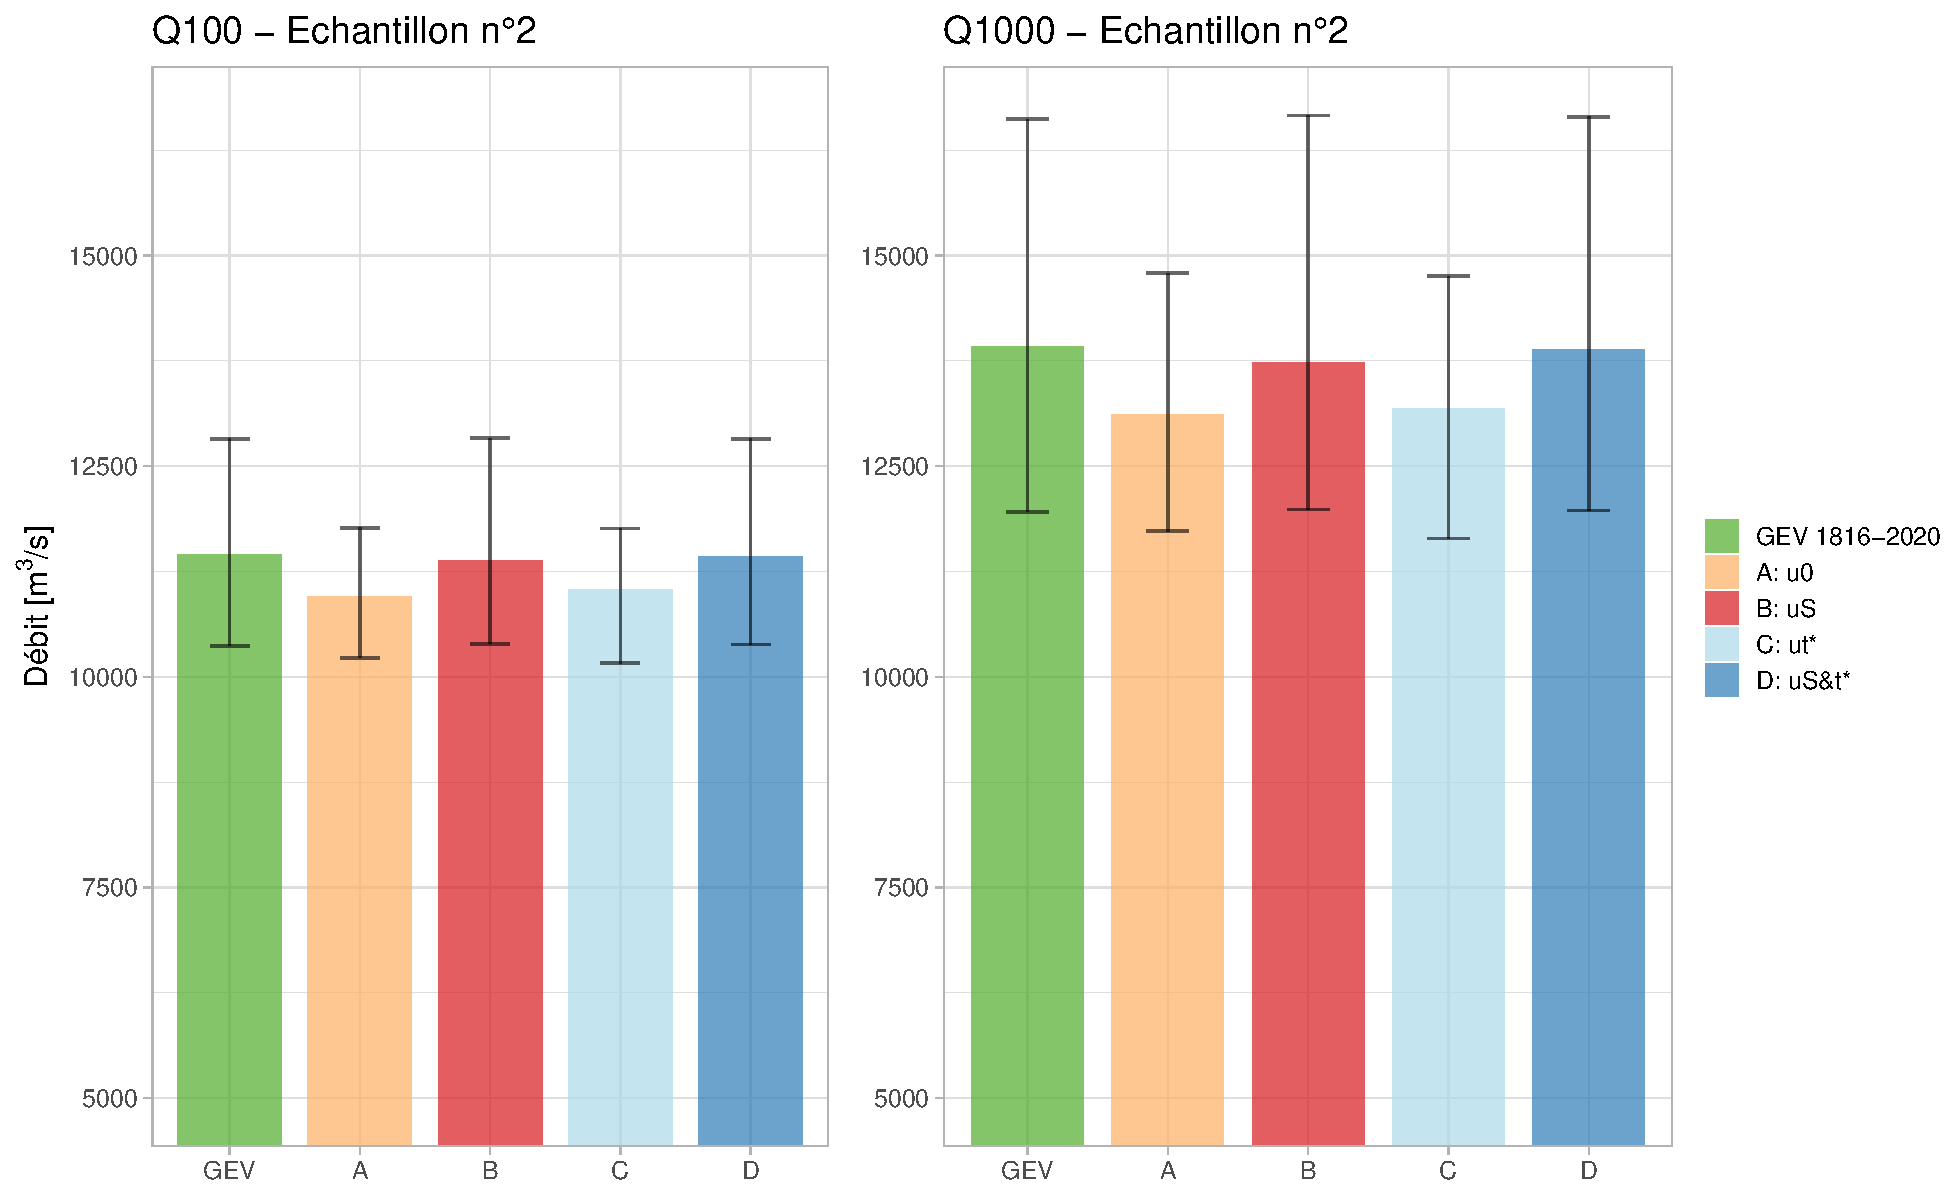
\includegraphics[width=.8\linewidth]{Figures/Barplots_QX_C4.pdf}
		\caption{Estimations maxpost et incertitudes à 95\% pour Q100 et Q1000 par 5 modèles différents pour l'échantillon 2 (1500-2020, $S4$)}
		\label{fig:BarplotC4}
	\end{figure}
	
	\paragraph{} La figure \ref{fig:QuantilesC4} permet de juger la cohérence des quantiles estimés par les modèles avec les observations de crues. Les estimations des 5 modèles semblent cohérentes avec les observations. (VRAIMENT UTILE ICI?)	
	
	\begin{figure}[h]
		\centering
		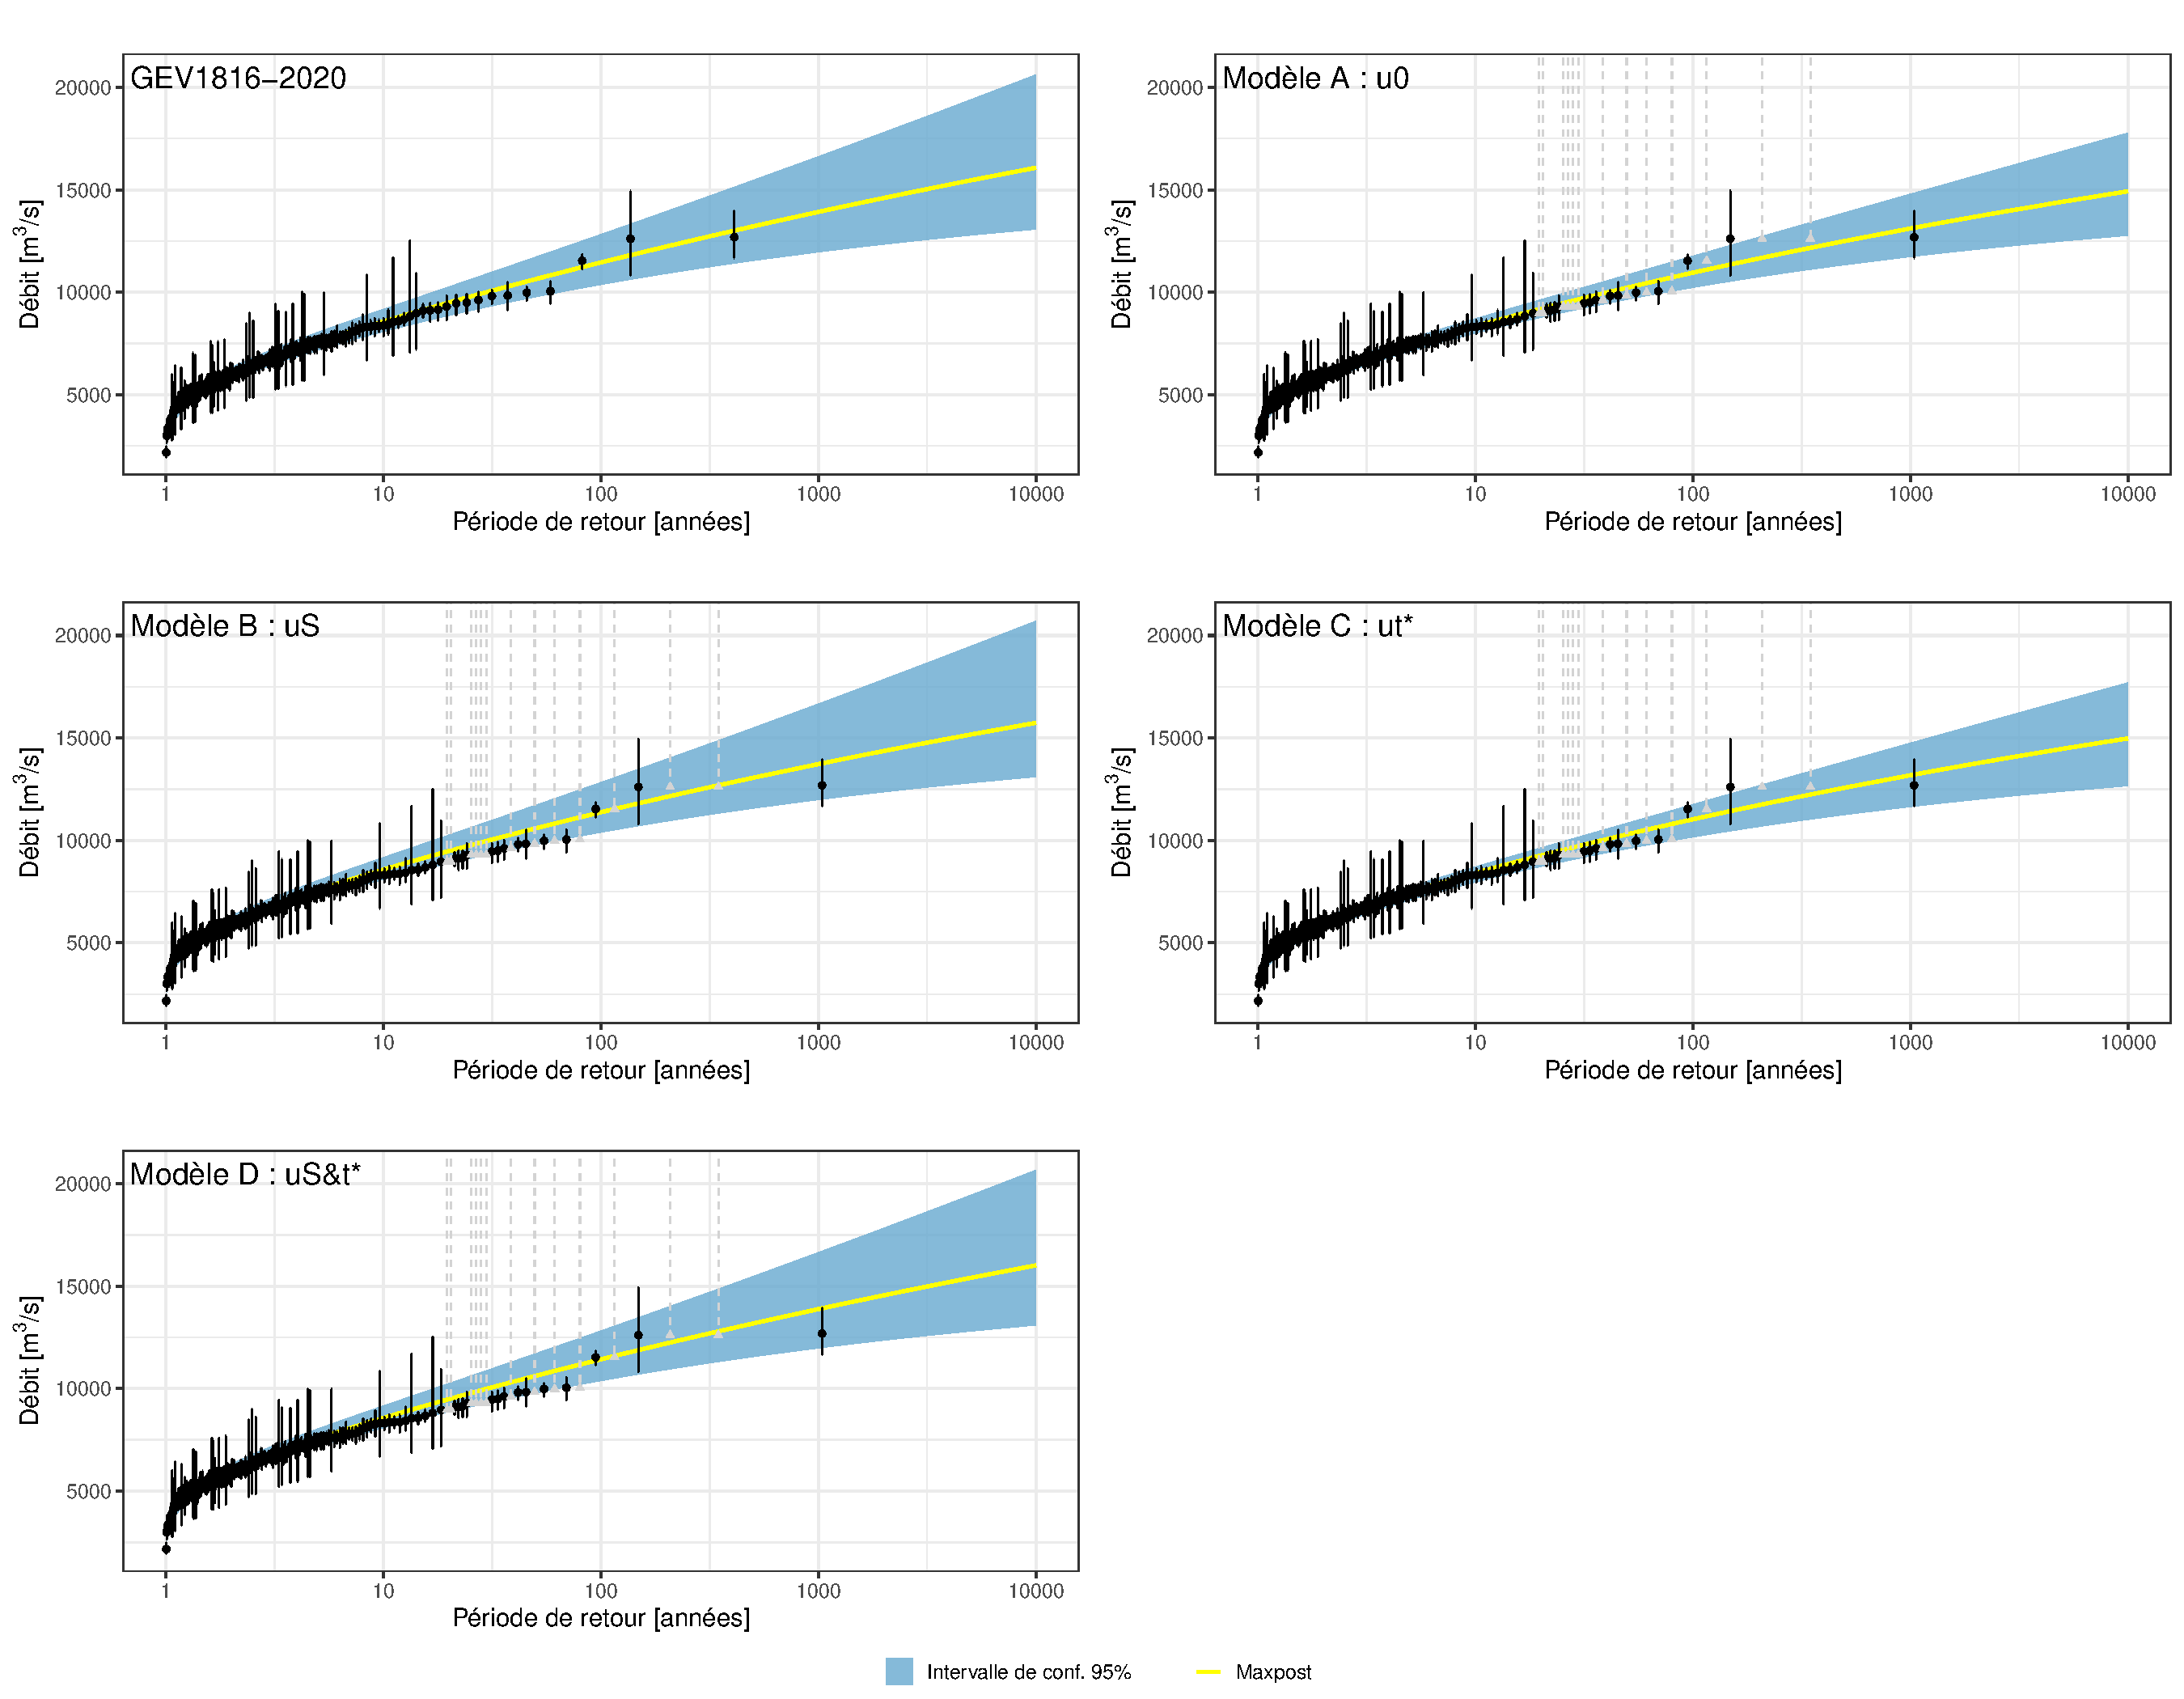
\includegraphics[width=.9\linewidth]{Figures/Quantiles_C4.pdf}
		\caption{Quantiles estimés par 5 modèles pour l'échantillon 2 (1500-2020, $S4$). Les observations sont en noir pour la période continue et en gris pour la période historique.}
		\label{fig:QuantilesC4}
	\end{figure}
	
	\paragraph{}Paramètre de forme
	
\begin{figure}[h]
		\centering
		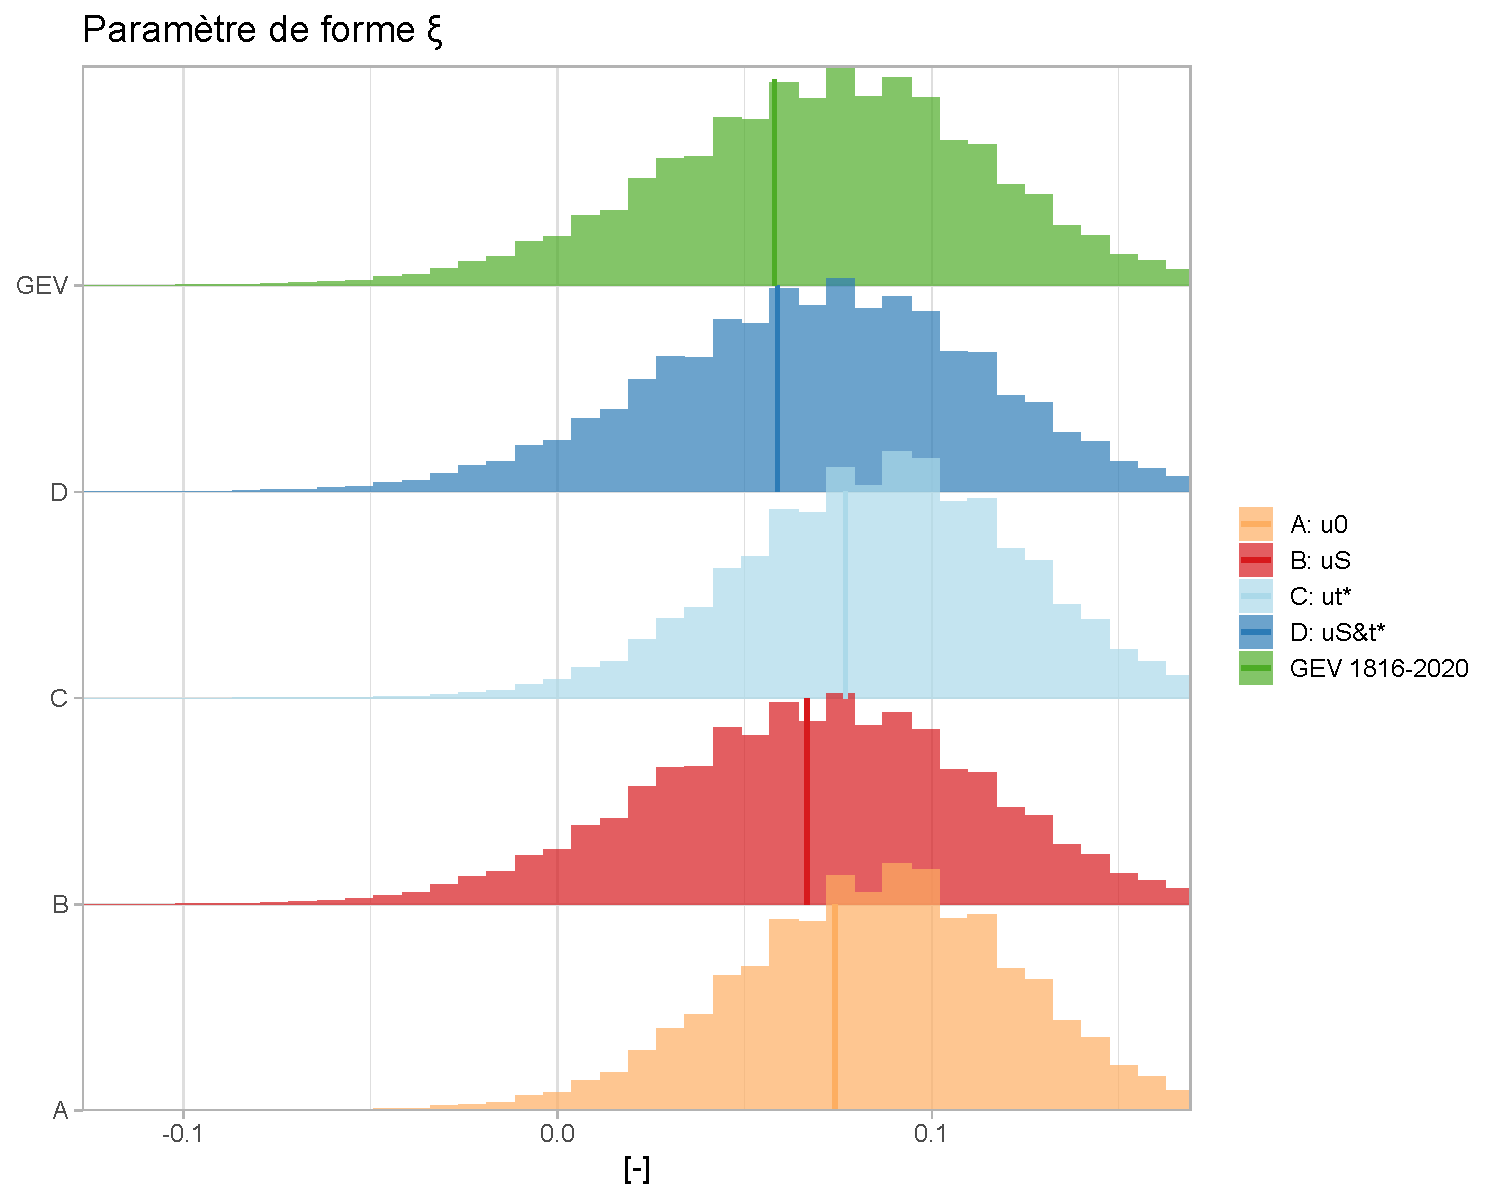
\includegraphics[width=.6\linewidth]{Figures/Shape_C4.pdf}	
		\caption{Distributions a posteriori du paramètre de forme pour les 4 modèles estimés sur l'échantillon 2. Les estimations des modèles GEV sont également indiquées. Les droites verticales représentent les valeurs maxpost.}
		\label{fig:Shape_C4}
	\end{figure}
	
	\paragraph{} Description \ref{fig:Params_C4}.
	
	
	\begin{figure}[h]
		\centering
		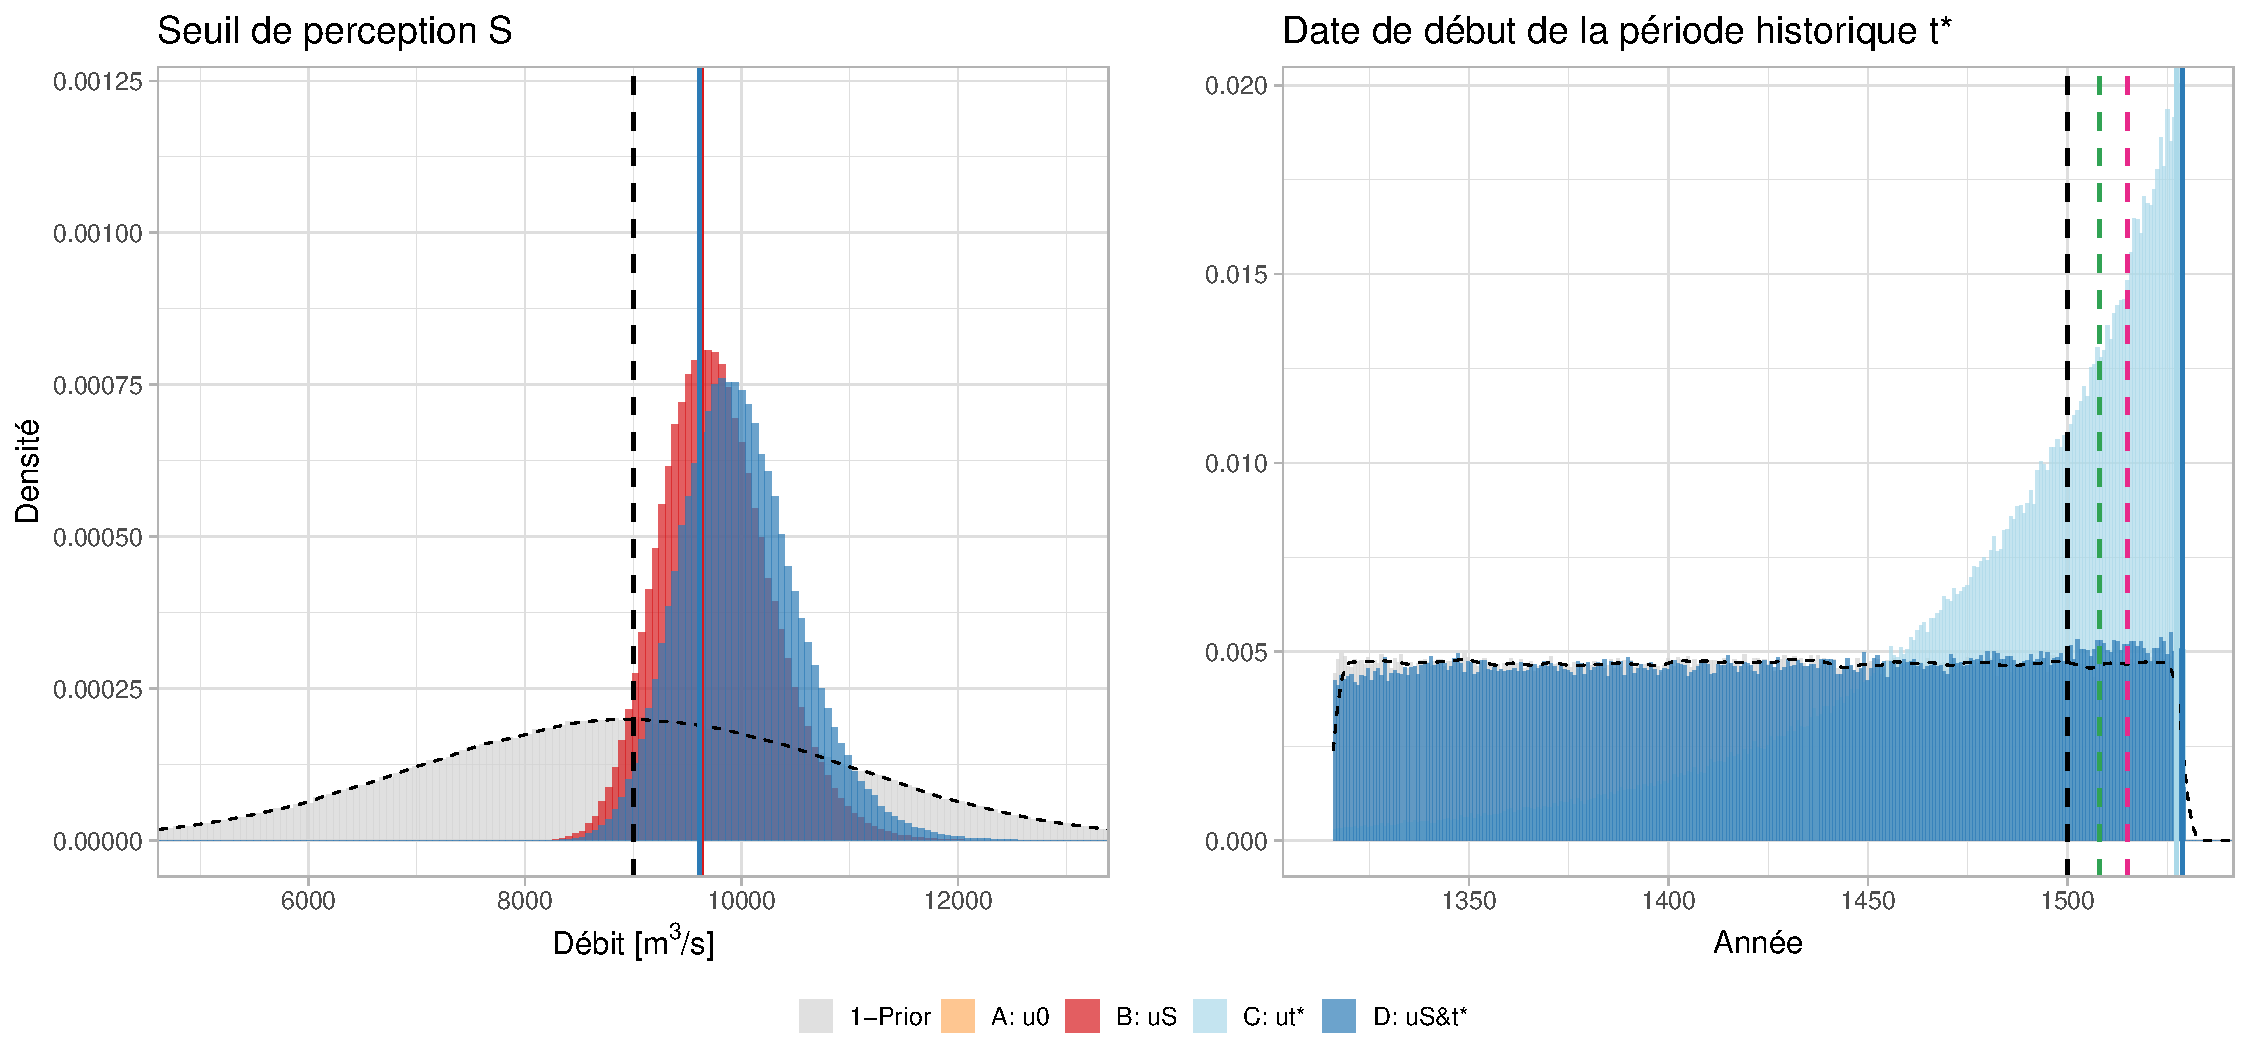
\includegraphics[width=.9\linewidth]{Figures/Params_C4.pdf}	
		\caption{Distributions a priori et a posteriori pour le seuil de perception (gauche) et la date de début de la période historique (droite). Les droites verticales représentent l'estimation maxpost du paramètre de forme pour chacun des modèles. La droite verticale noire représente la date de début supposée de la chronique historique, ici 1500.}
		\label{fig:Params_C4}
	\end{figure}
	
	\paragraph{} maxpost début période histo = 1530\\
	Pourquoi seuil $\geq$ 9000 et Nban supérieur à 1500. 
	Il manque des crues dans la période historique VS la période continue. Remise en cause des résultats de Pichard. 
	
		\subsubsection{Quel est l'apport des crues historiques pour l'analyse fréquentielle à Beaucaire ?}

	 De la même manière qu'avec l'échantillon dégradé, on observe ici que la méconnaissance du seuil de perception (B et D) a plus d'impact sur l'incertitude des résultats que la méconnaissance de la durée de la période historique (C et D). De plus, l'incertitude autour des résultats est plus faible que celle de la référence uniquement dans les cas où le seuil de perception est supposé connu (modèles A et C). L'utilisation du nombre d'occurrences de crues historiques supérieures à un seuil ne permet de réduire l'incertitude autour des quantiles estimés qu'à la condition de la connaissance du seuil de perception. (attention, prior très large QUID avec un prior plus serré?)


	
		\subsubsection{Modèle A pour les échantillons 1 et 2 : Quel est l'impact du choix de l'échantillon de crues historiques (S3 vs S4)}
%	Comparaison des résultats du modèle (A) pour les échantillon ("C3 \& C4") et ("C4")\\
%	Barplot Q100 et Q1000	
	
%		\subsubsection{Quel est l'impact de la méconnaissance du seuil de perception ?}
%	Comparaison des résultats du modèle (A) et du modèle (B) pour l'échantillon ("C3 \& C4")\\
%	Barplot Q100 et Q1000, et comparaison de la distribution a postériori du seuil
	
%		\subsubsection{Quel est l'impact de la méconnaissance de la durée de la période historique ?}
	
%	Comparaison des résultats du modèle (B) et du modèle (C) pour l'échantillon ("C3 \& C4")\\
%	Barplot Q100 et Q1000, comparaison de la distribution a postériori du seuil et de la taille de la période historique\\
%	Comparaison de la date de début de la période historique estimée par le modèle (maxpost) avec la date obtenue via la méthode de \cite{prosdocimi_german_2018}.\\
	
	\FloatBarrier
	
	\subsection{Discussion}
	
	Il manque des crues dans la base histrhône
	
\section{Conclusion du chapitre}
	Conclusions sur l'intérêt des crues historiques pour l'estimation des quantiles extrêmes à Beaucaire. \\
	Est-ce qu'on observe une réelle amélioration par rapport aux résultats du chapitre 1 ?\\
	Selon les résultats, ajouter quelque chose comme : "l'utilisation des crues historiques peut mener à faire de fortes hypothèses (seuil et durée de la période), il faut être pragmatique sur la considération des incertitudes, même si elles mènent à des estimations incertaines des quantilese\\
	Ces conclusions sont valables uniquement à Beaucaire (période continue très longue, paramètre de forme positif, pas de tendance observée due au changement climatique ou autre). Mais que nous a appris l'application du modèle à un échantillon dégradé plus représentatif des longueurs de chronique habituelles ?\\
	Les a priori données ici sont très peu informatifs. Des a priori plus informatifs peuvent être élicités (comment ? Courbe de tarage Beaucaire / Arles, modélisation ,...) \\
	Perspectives sur les modèles d'analyse fréquentielle en contexte non-stationnaire et sur les modèles régionaux.  

\printbibliography[title=Bibliographie]
\end{document}
